\section{Analysis}

\subsection{Analysis of F2}
For analysis the F2 process step contained the significantly more data compared to F4 and F5 which makes the results somewhat more reliable. However, since the sample size is nevertheless small, the results need to be taken as inconclusive and in need of additional research and interpretation by someone with deep knowledge of the process. It should be noted, that the classification into rejected, released and restricted release categories is not balanced with most of the data residing in release category. This is naturally reflected in the distribution of the data as depicted in Figure \ref{fig:f2_sample}. This figure does not include time series that are either static or otherwise lack significant information. 

It is immediately evident, that in most time series, the batches that were later classified as ``rejected'' contain significantly more variance than the other two categories. This cannot be explained by just other categories having different quantities of data.

\begin{figure}[ht]
    \centering
    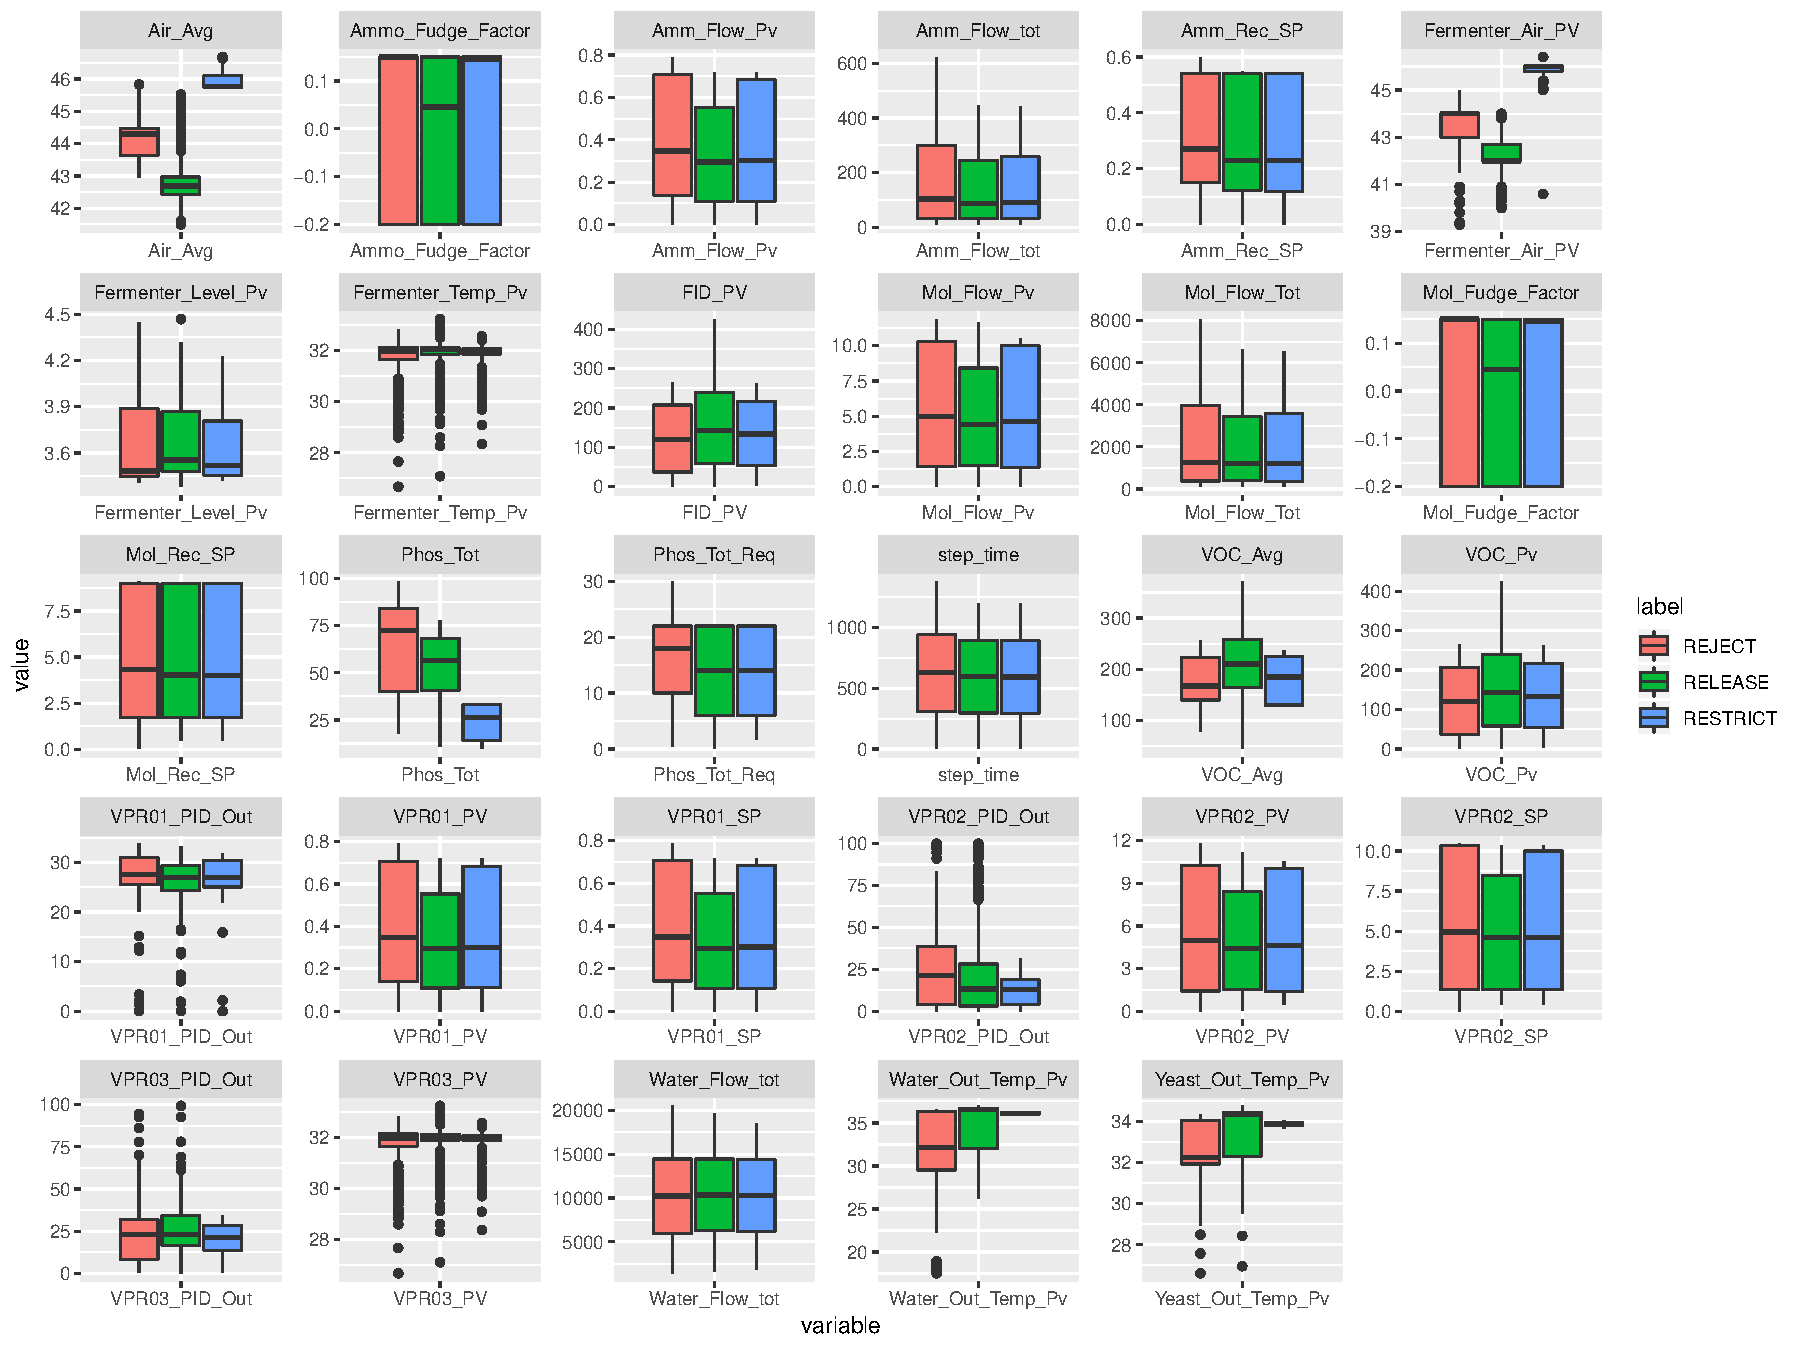
\includegraphics[width=1.0\textwidth]{plots/f2-sample.pdf}
    \caption{F2 sample}
    \label{fig:f2_sample}
\end{figure}

This pattern continued after normalizing the variables to a common scale and performing PCA feature reduction and LDA clustering. As can be seen from Figure \ref{fig:f2_predicted}, also the predicted labels of the production batches follow the same trend of ``rejected'' having significantly larger amount of variance. Since as of this writing, the authors lack profound knowledge about the process, it is difficult to say, if the claim, that variance in F2 process parameters is the cause of undesired mutations, has any substance. However, we believe, that there is enough evidence to do additional research on the effects of F2 process stability on the quality of the yeast.

\begin{figure}[ht]
    \centering
    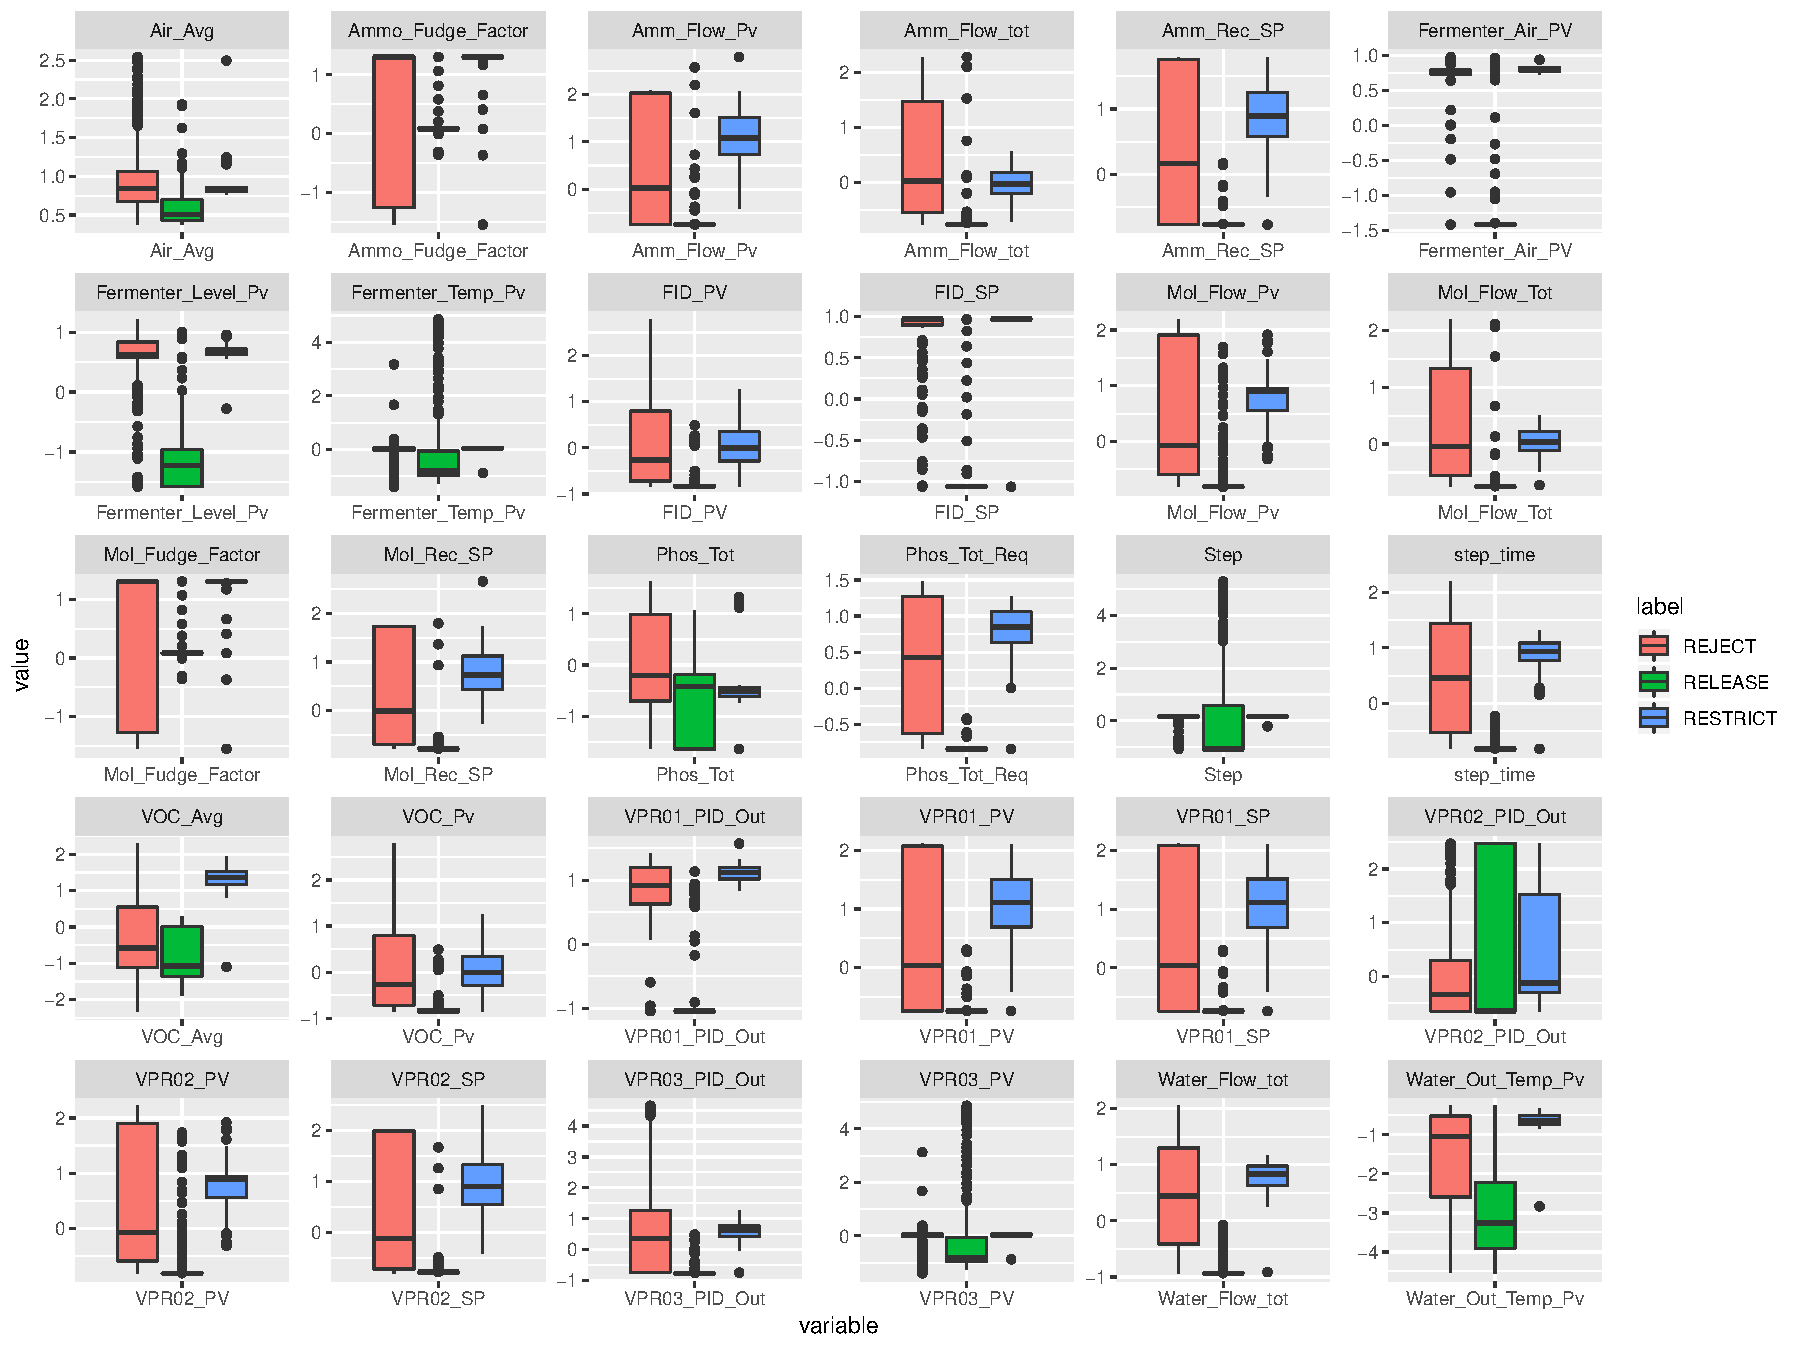
\includegraphics[width=1.0\textwidth]{plots/f2-predicted.pdf}
    \caption{F2 predicted}
    \label{fig:f2_predicted}
\end{figure}

When looking at the effectiveness of feature reduction and clustering, then, as it can be easily seen from Figure \ref{fig:f2_explained_variances}, most of the variance in F2 process data can be explained the one factor, with first 3 factors explaining more than 90\% of the variance in the process data. That indicates that there are strong correlations between parallel time series in the process that can be aggregated into smaller number of series with highly similar explanatory power. Moreover, Figure \ref{fig:f2_variables} also shows a strong clustering indicating correlations and need for feature reduction.

Therefore, when looking only the feature reduced data and investigating the first, by far, the most significant factor, it is evident, that the ``rejected'' and ``release'' batches are indeed different. See Figure \ref{fig:f2_LD1} for detailed representation. Therefore we believe that the process of F2 should be further investigated.

\begin{figure}
    \begin{subfigure}{0.3\textwidth}
        \begin{center}
        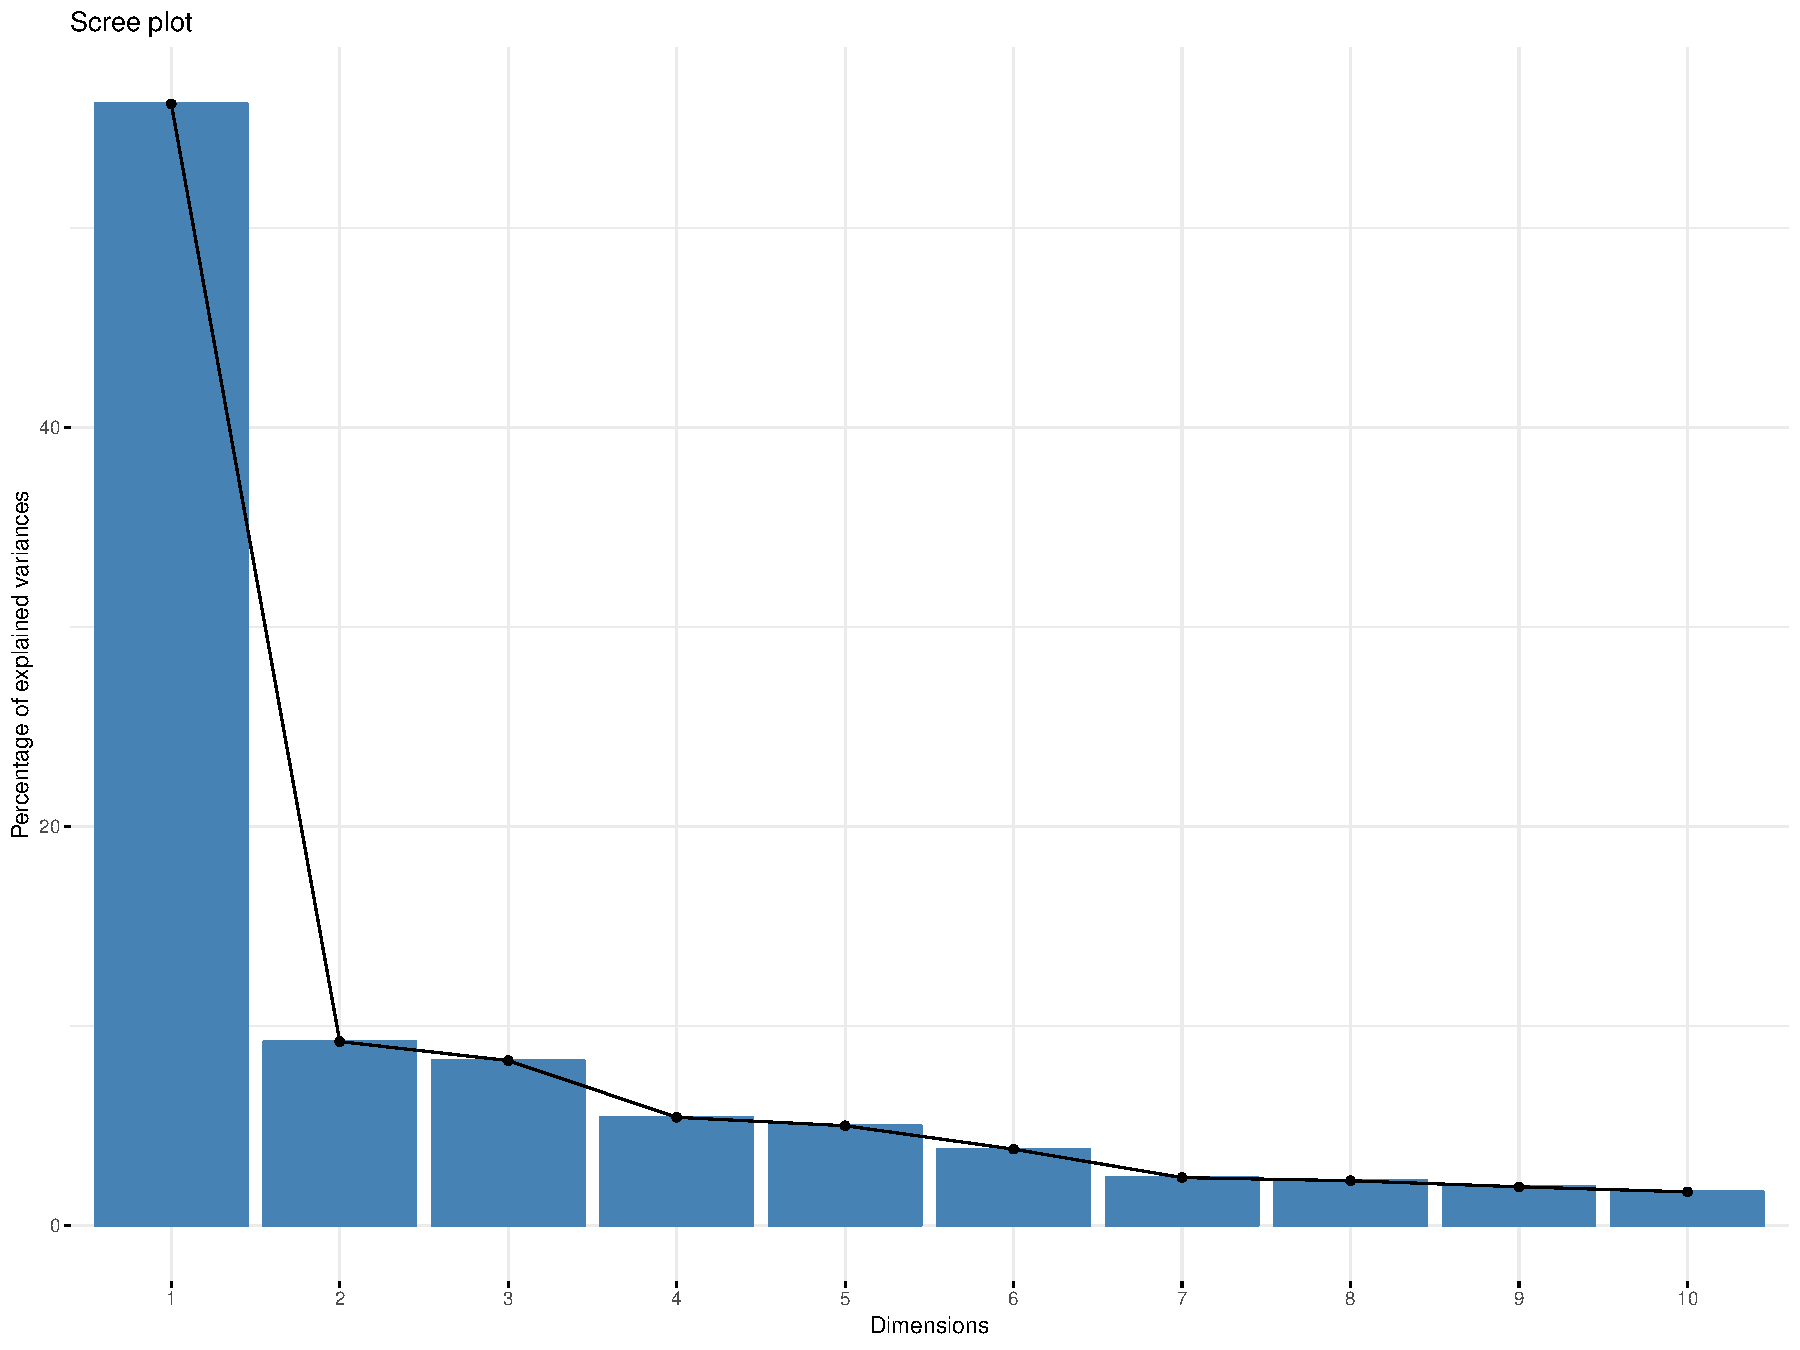
\includegraphics[width=\textwidth]{plots/f2_explained_variances.pdf}        
        \end{center}
        \caption{F2 explained variances}
        \label{fig:f2_explained_variances}
    \end{subfigure}%
    \begin{subfigure}{0.3\textwidth}
        \begin{center}
        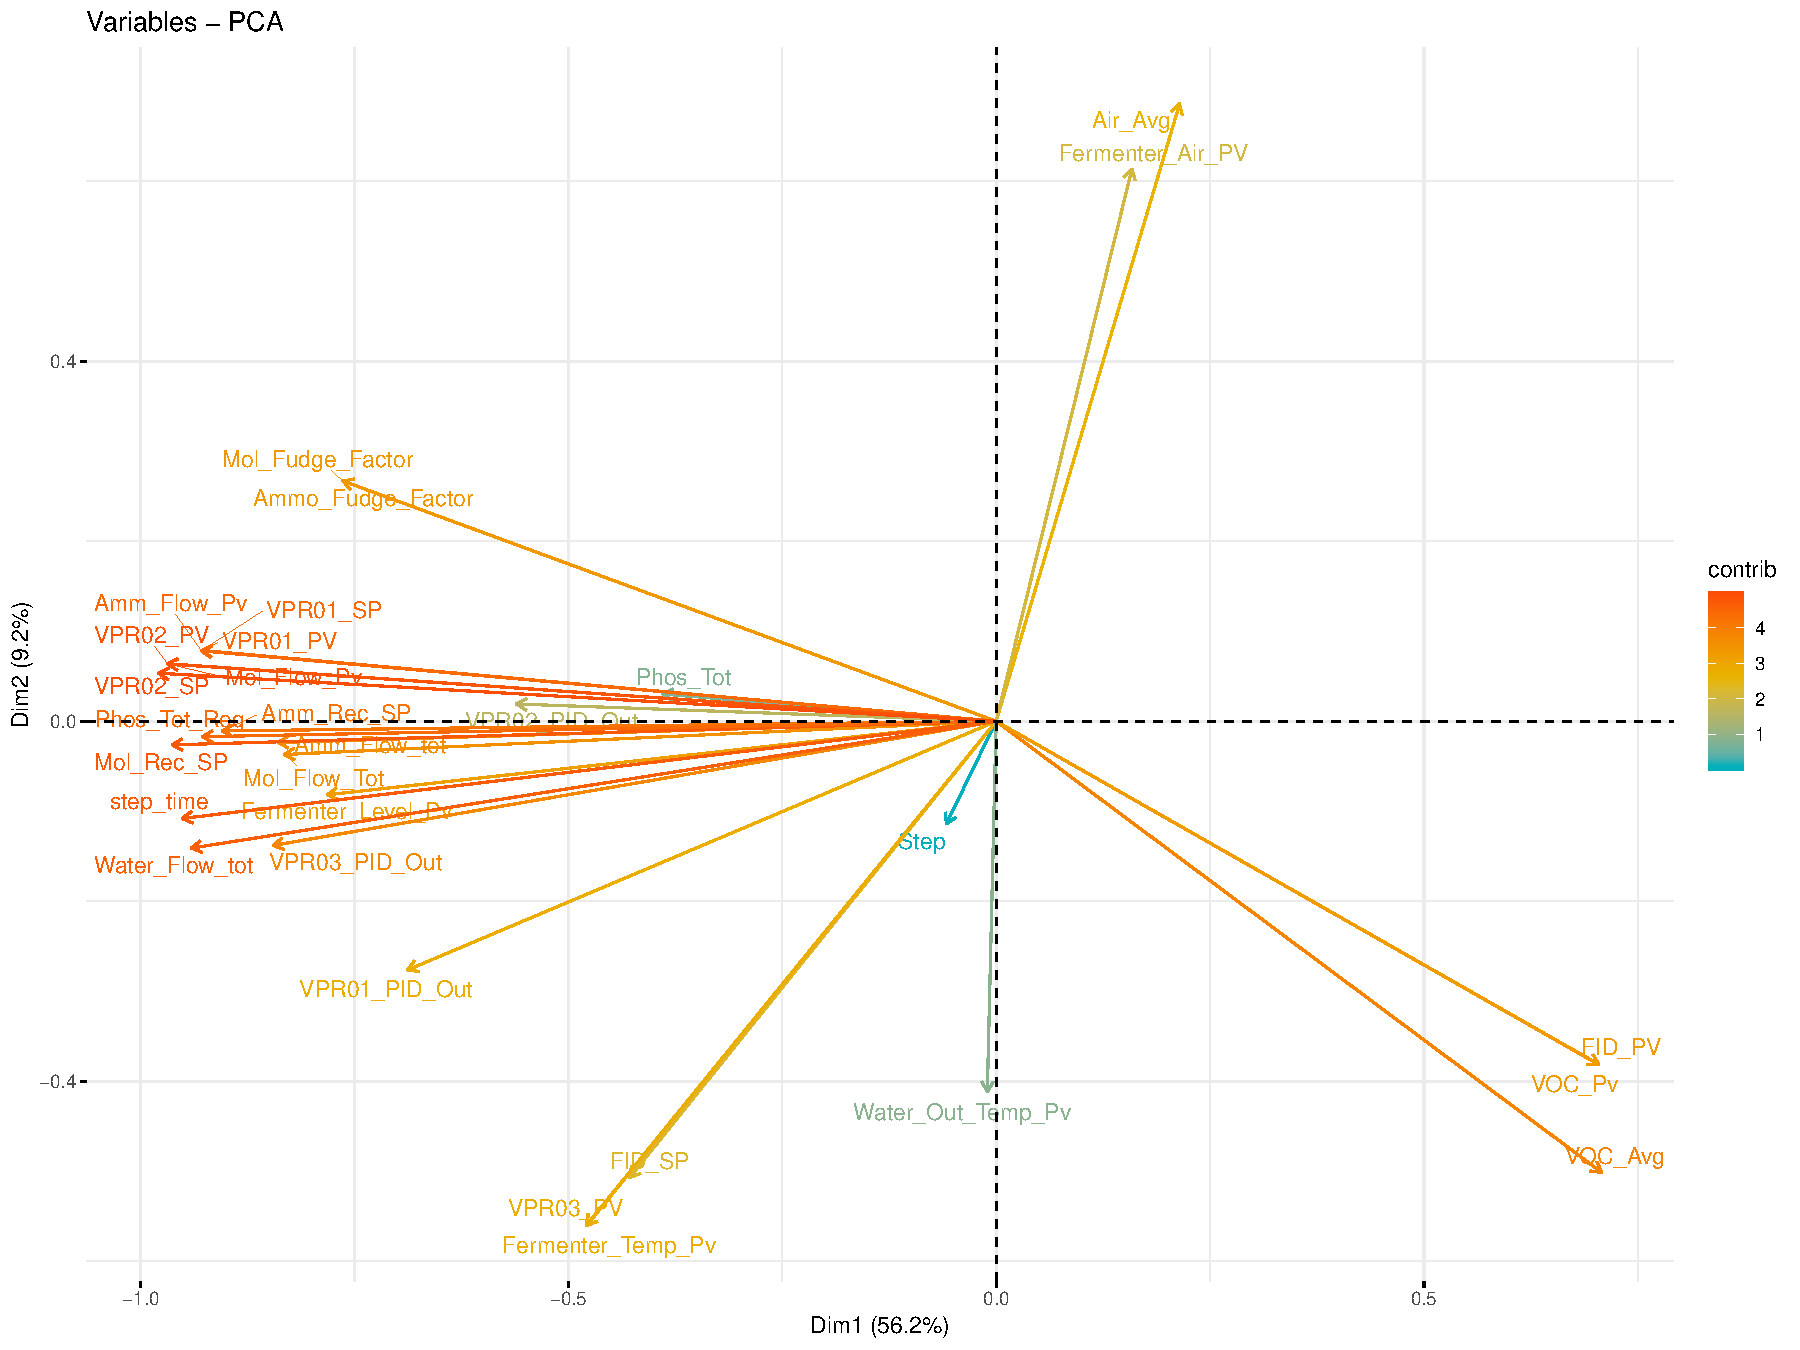
\includegraphics[width=\textwidth]{plots/f2_graph_of_variables.pdf}
        \end{center}
        \caption{F2 Variables}
        \label{fig:f2_variables}
    \end{subfigure}%
    \begin{subfigure}{0.3\textwidth}
        \begin{center}
        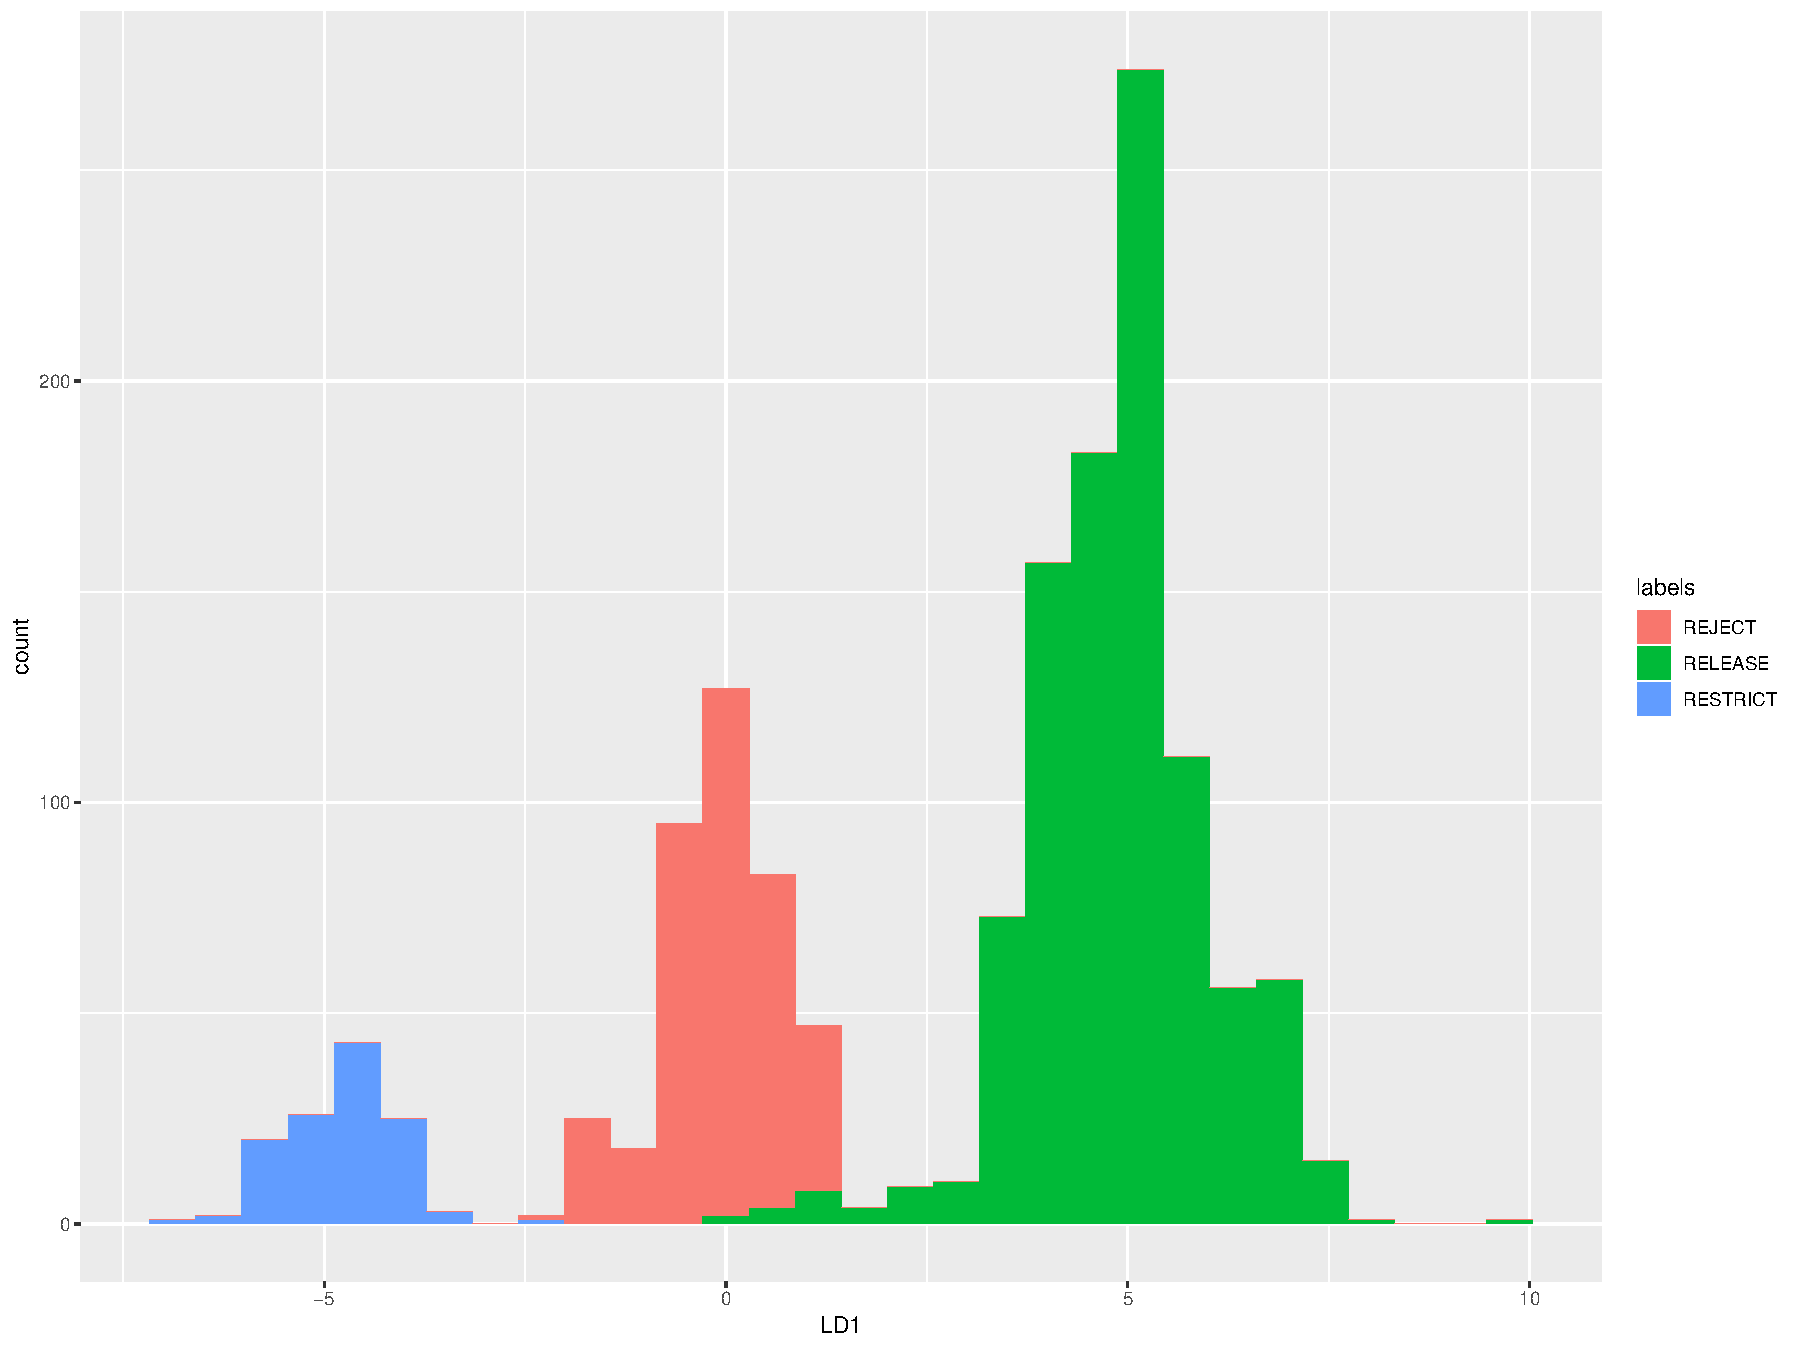
\includegraphics[width=\textwidth]{plots/f2_LD1.pdf}
        \end{center}
        \caption{F2 LD1 distribution across classes}
        \label{fig:f2_LD1}
    \end{subfigure}
\end{figure}


\subsection{Analysis of F4}
The analysis of step F4 was performed similarly to the step F2 above. We investigated the variance of data to see the potential differences between the classes. Then we performed PCA and LDA to investigate the clustering of the data and to see whether the differences between the clusters are indeed significant.

Compared to F5, F4 was relatively well populated data set. Again, the main weakness lies within the uneven balance between ``released'' and ``rejected'' classes. Therefore, the conclusions and results of the analysis are statistically weak and either need to be improved by additional data collection and experimentation of significant injection of process knowledge. As it is evident from the box plot of the data depicted on Figure \ref{fig:f4_sample}, the difference between three classes of batches appears to be insignificant. Most medians of the time series are close to each other and the variance of the 25\% and 75\% percentiles can be explained by a few number of random observations that have shifted the percentile cutoff points. 

\begin{figure}[ht]
    \centering
    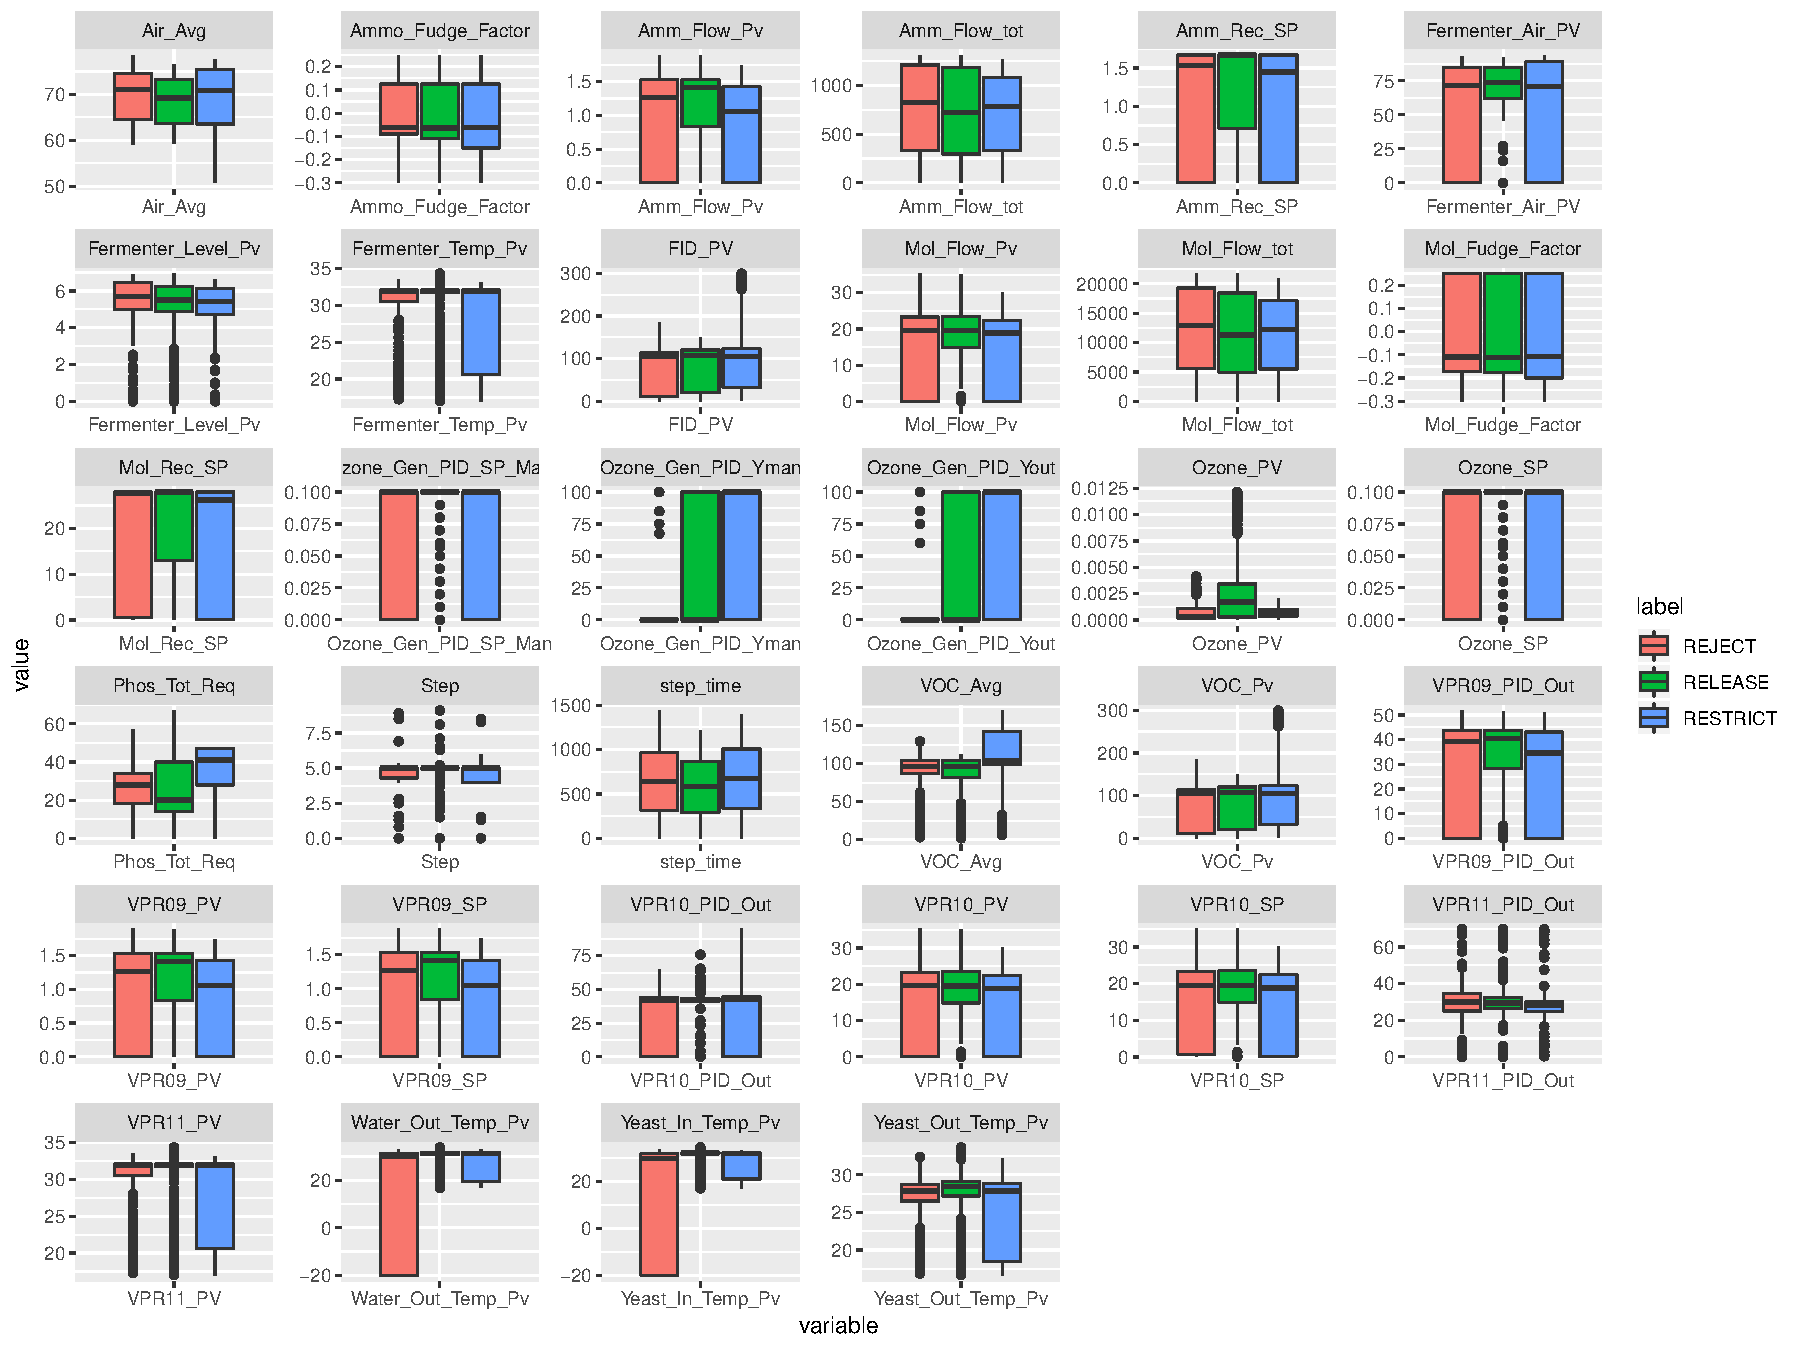
\includegraphics[width=1.0\textwidth]{plots/f4-sample.pdf}
    \caption{F4 sample}
    \label{fig:f4_sample}
\end{figure}

Similar picture can be seen with modelled data and predicted labels shown at Figure \ref{fig:f2_predicted}, no significant difference exists, the only differentiator here compared to the previous figure is, that due to the similarity, the predictive power of the model is low and thus the data points have received erroneous labels from the model with a significant amount of ``rejected'' category data points being labelled as ``released''.

\begin{figure}[ht]
    \centering
    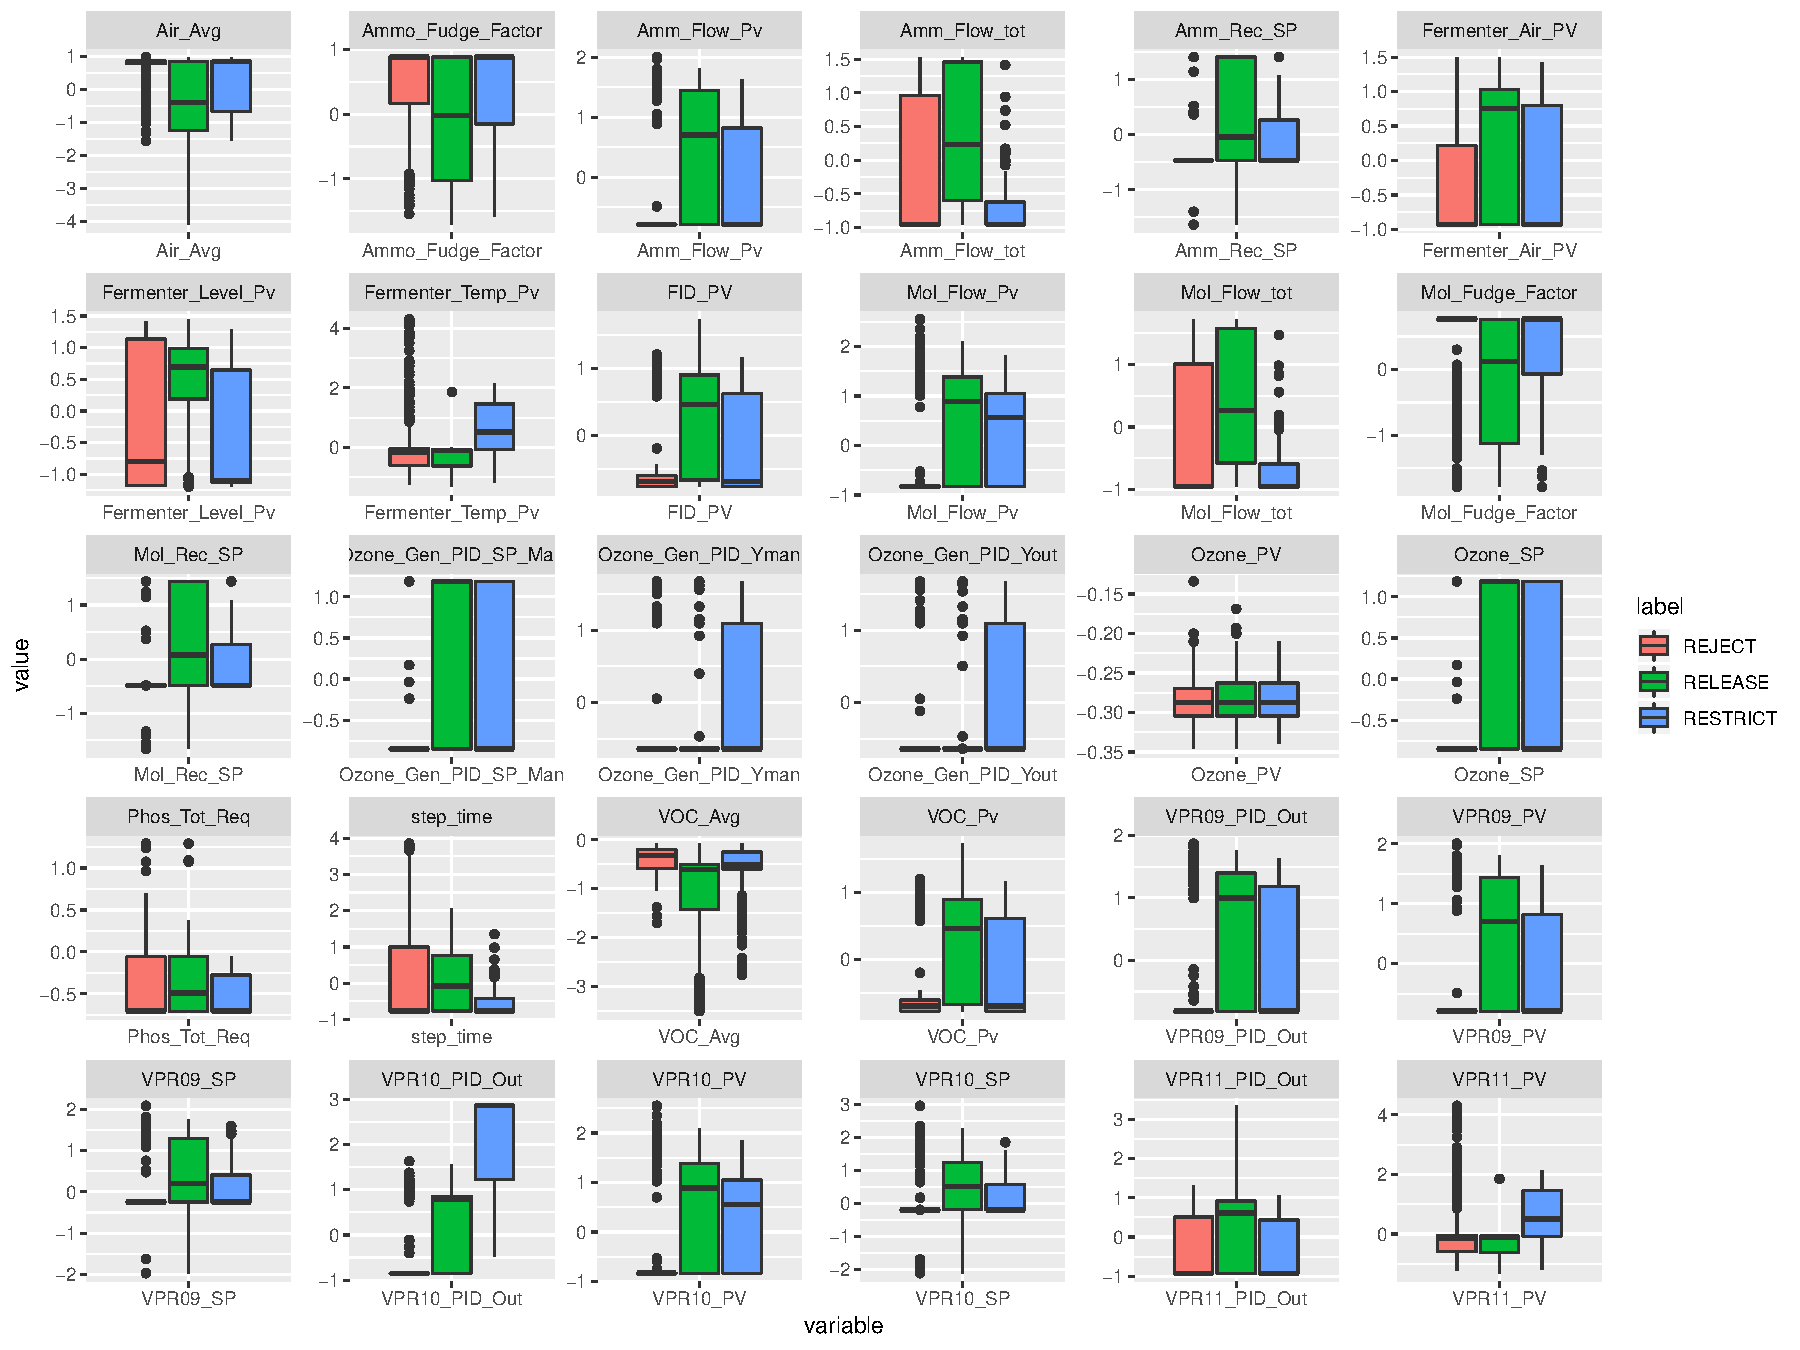
\includegraphics[width=1.0\textwidth]{plots/f4-predicted.pdf}
    \caption{F4 predicted}
    \label{fig:f4_predicted}
\end{figure}

When looking at the results of PCA and LDA, then the results of PCA are significant. Again, due to strong correlations between parallel time series, the data can be significantly feature reduced. The effect of PCA as displayed on Figure \ref{fig:f4_explained_variances} is significant, with first 3 components explaining well over 90\% of the variance in the time series. That, similarly to F2, is supported by strong clustering of process variables as evident on Figure \ref{fig:f4_variables}. Correlations between the time series create one significant cluster (LD1 axis positive values) and two smaller clusters in $3^{rd}$ and $4^{th}$ quadrants of the chart.

\begin{figure}
    \begin{subfigure}{0.3\textwidth}
        \begin{center}
            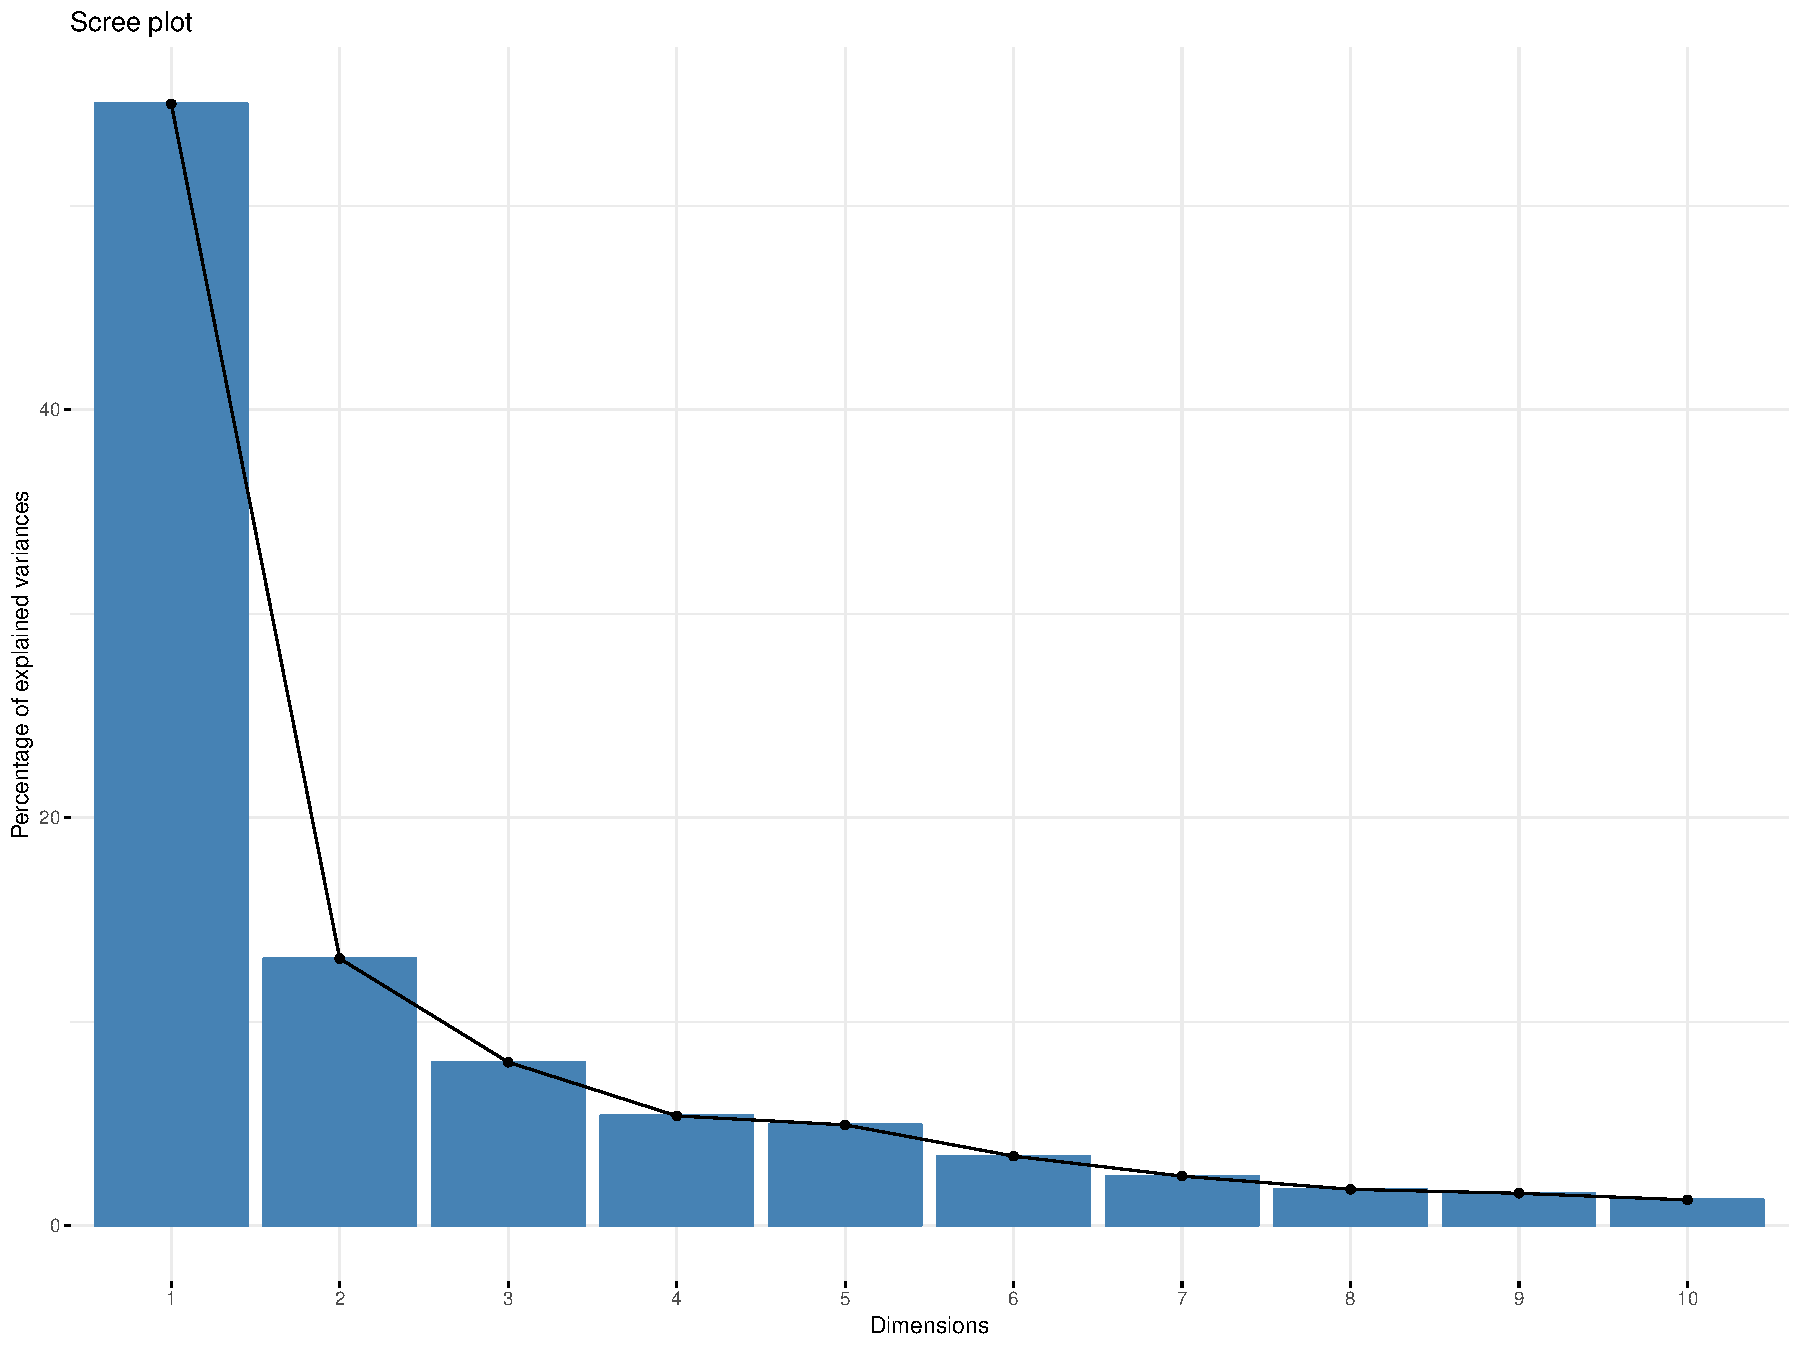
\includegraphics[width=\textwidth]{plots/f4_explained_variances.pdf}        
        \end{center}
        \caption{F4 explained variances}
        \label{fig:f4_explained_variances}
    \end{subfigure}%
    \begin{subfigure}{0.3\textwidth}
        \begin{center}
        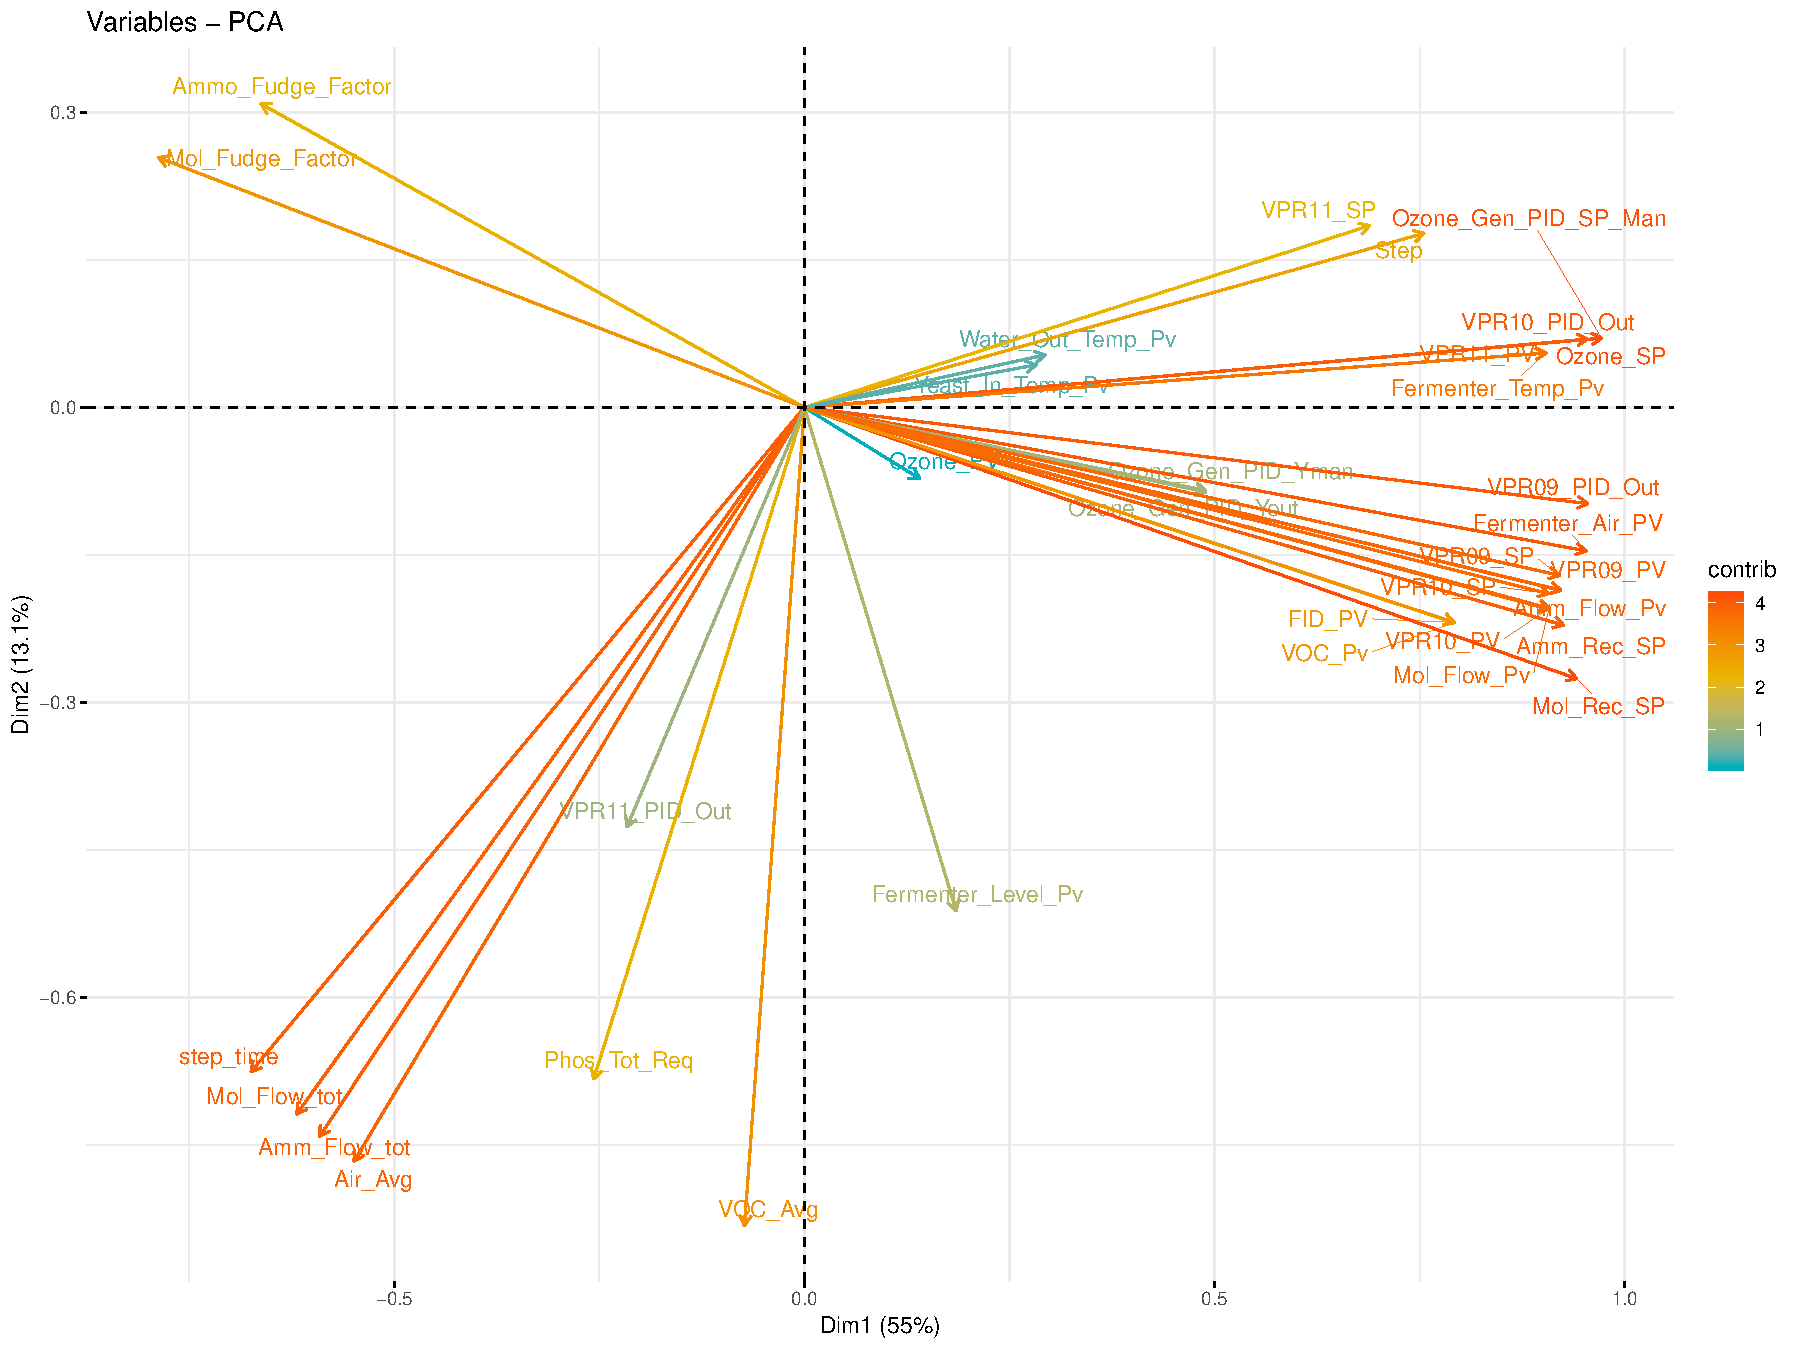
\includegraphics[width=\textwidth]{plots/f4_graph_of_variables.pdf}
        \end{center}
        \caption{F4 Variables}
        \label{fig:f4_variables}
    \end{subfigure}%
    \begin{subfigure}{0.3\textwidth}
        \begin{center}
        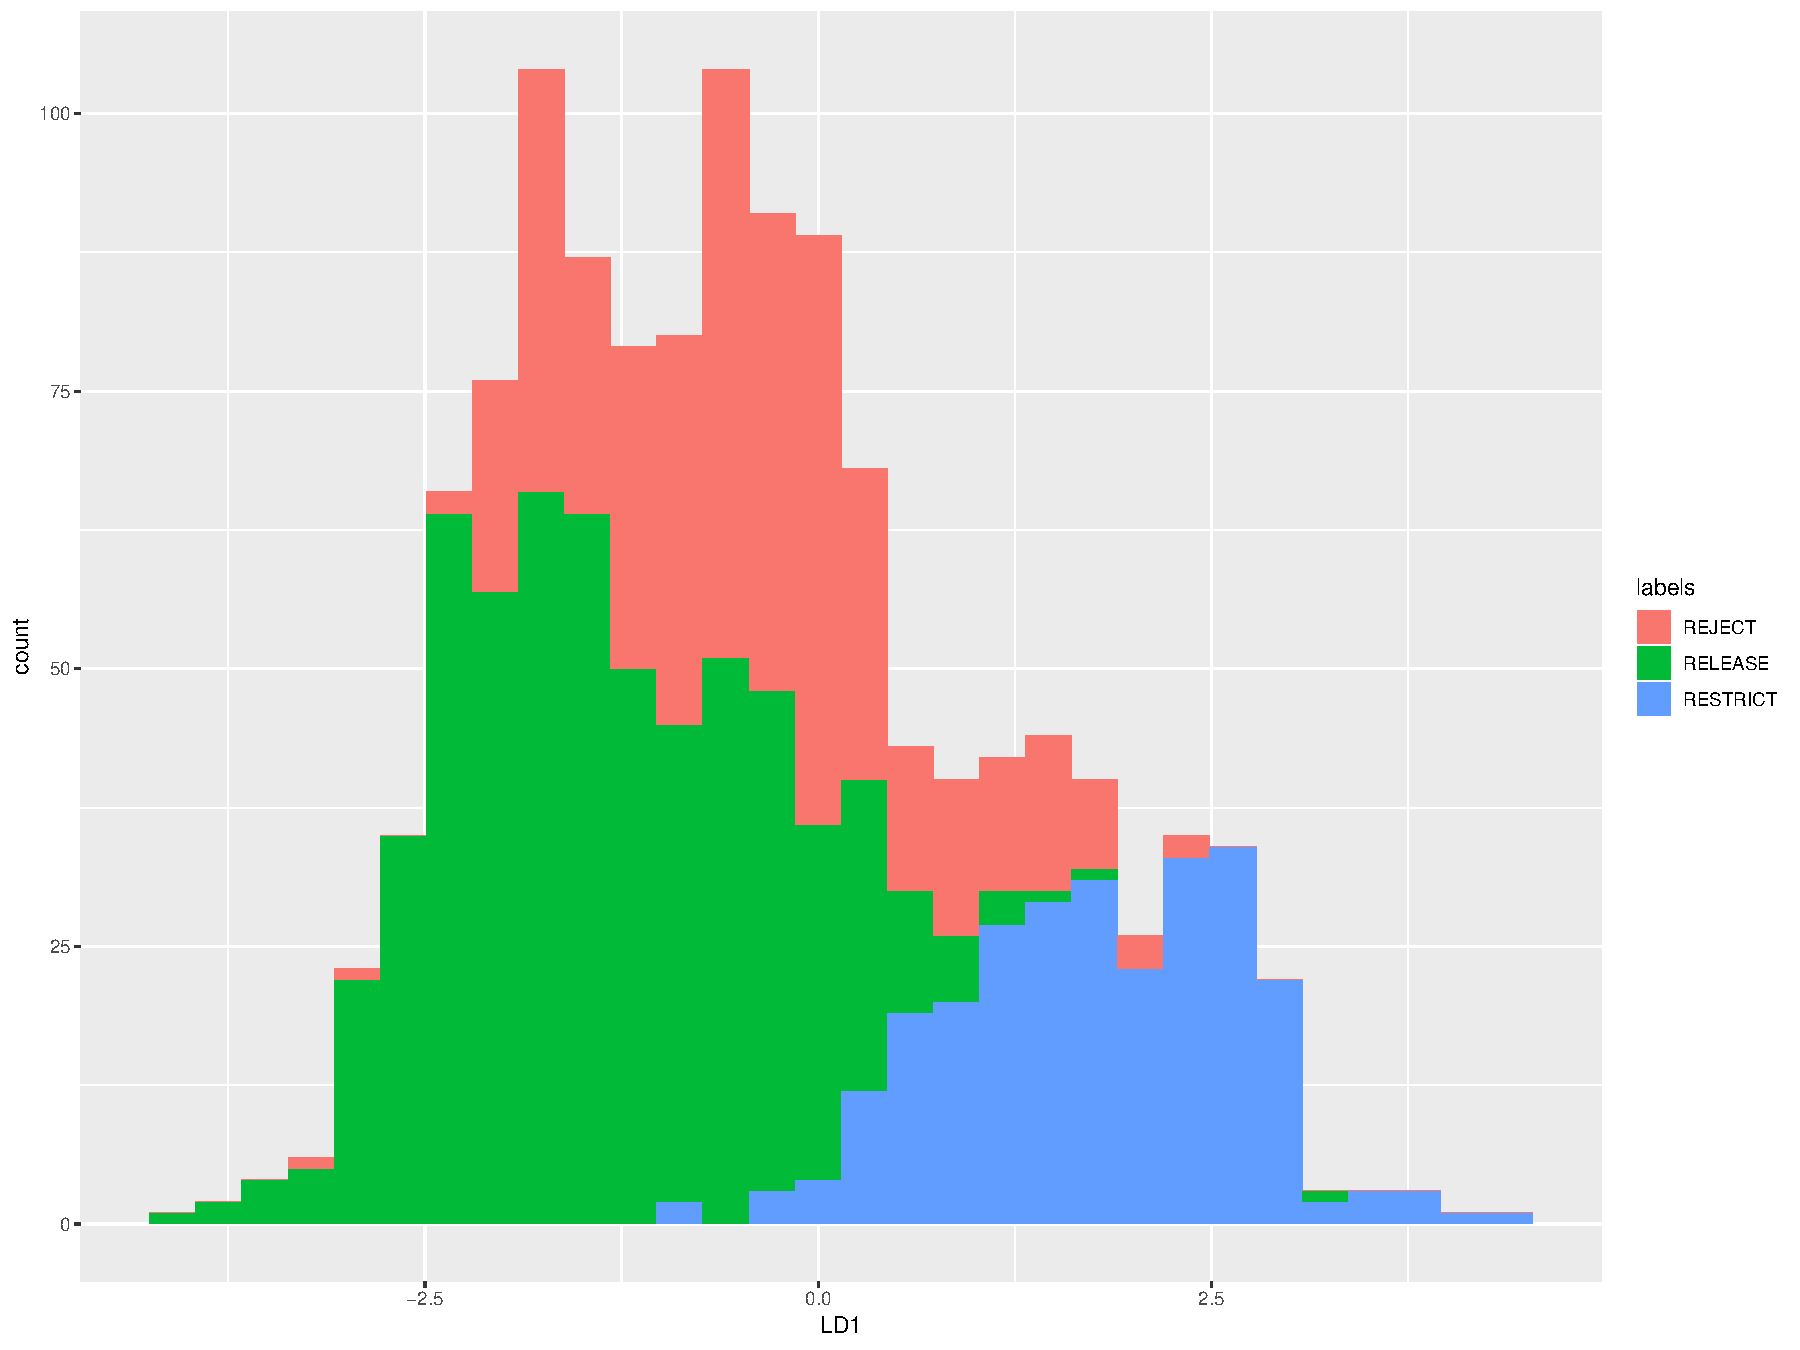
\includegraphics[width=\textwidth]{plots/f4_LD1.pdf}
        \end{center}
        \caption{F4 LD1 distribution across classes}
        \label{fig:f4_LD1}
    \end{subfigure}
\end{figure}

Nevertheless, LDA clustering was able to differentiate poorly between the three classes of batches as can be seen on Figure \ref{fig:f2_LD1}. It should be noted, that since the sample sizes are low, the differentiation can be random, ie. the LDA shows significant difference, because for whatever reason (environment, randomness, other nuisance factors) a few batches have different parametric data because the automation and process control system has behaved differently. Additional data and process knowledge are obviously needed before making and in-depth conclusions.

\subsection{Analysis of F5}
Lastly we performed the same analysis steps on F5. Before going any further, it should be noted, that since we had only two samples in F5 - one rejected and one release, then the results of the analysis are far for conclusive, lack strong statistical significance and are indicative at best. 

As it can be seen from box plots at Figure \ref{fig:f5_sample}, the process data with its medians, 25\% and 75\% percentiles varying with no clear pattern. Again, as with analysis of F2 and F4, the plot does not depict time series that were either constant or otherwise lacking explanatory information. It should be noted, that there is an interesting behaviour regarding air (\texttt{Air\_PID\_Out} and \texttt{Air\_PV}), ammonia (\texttt{Amm\_Flow\_Tot}) and molasses (\texttt{Mol\_Flow\_Tot}). 

\begin{figure}[ht]
    \centering
    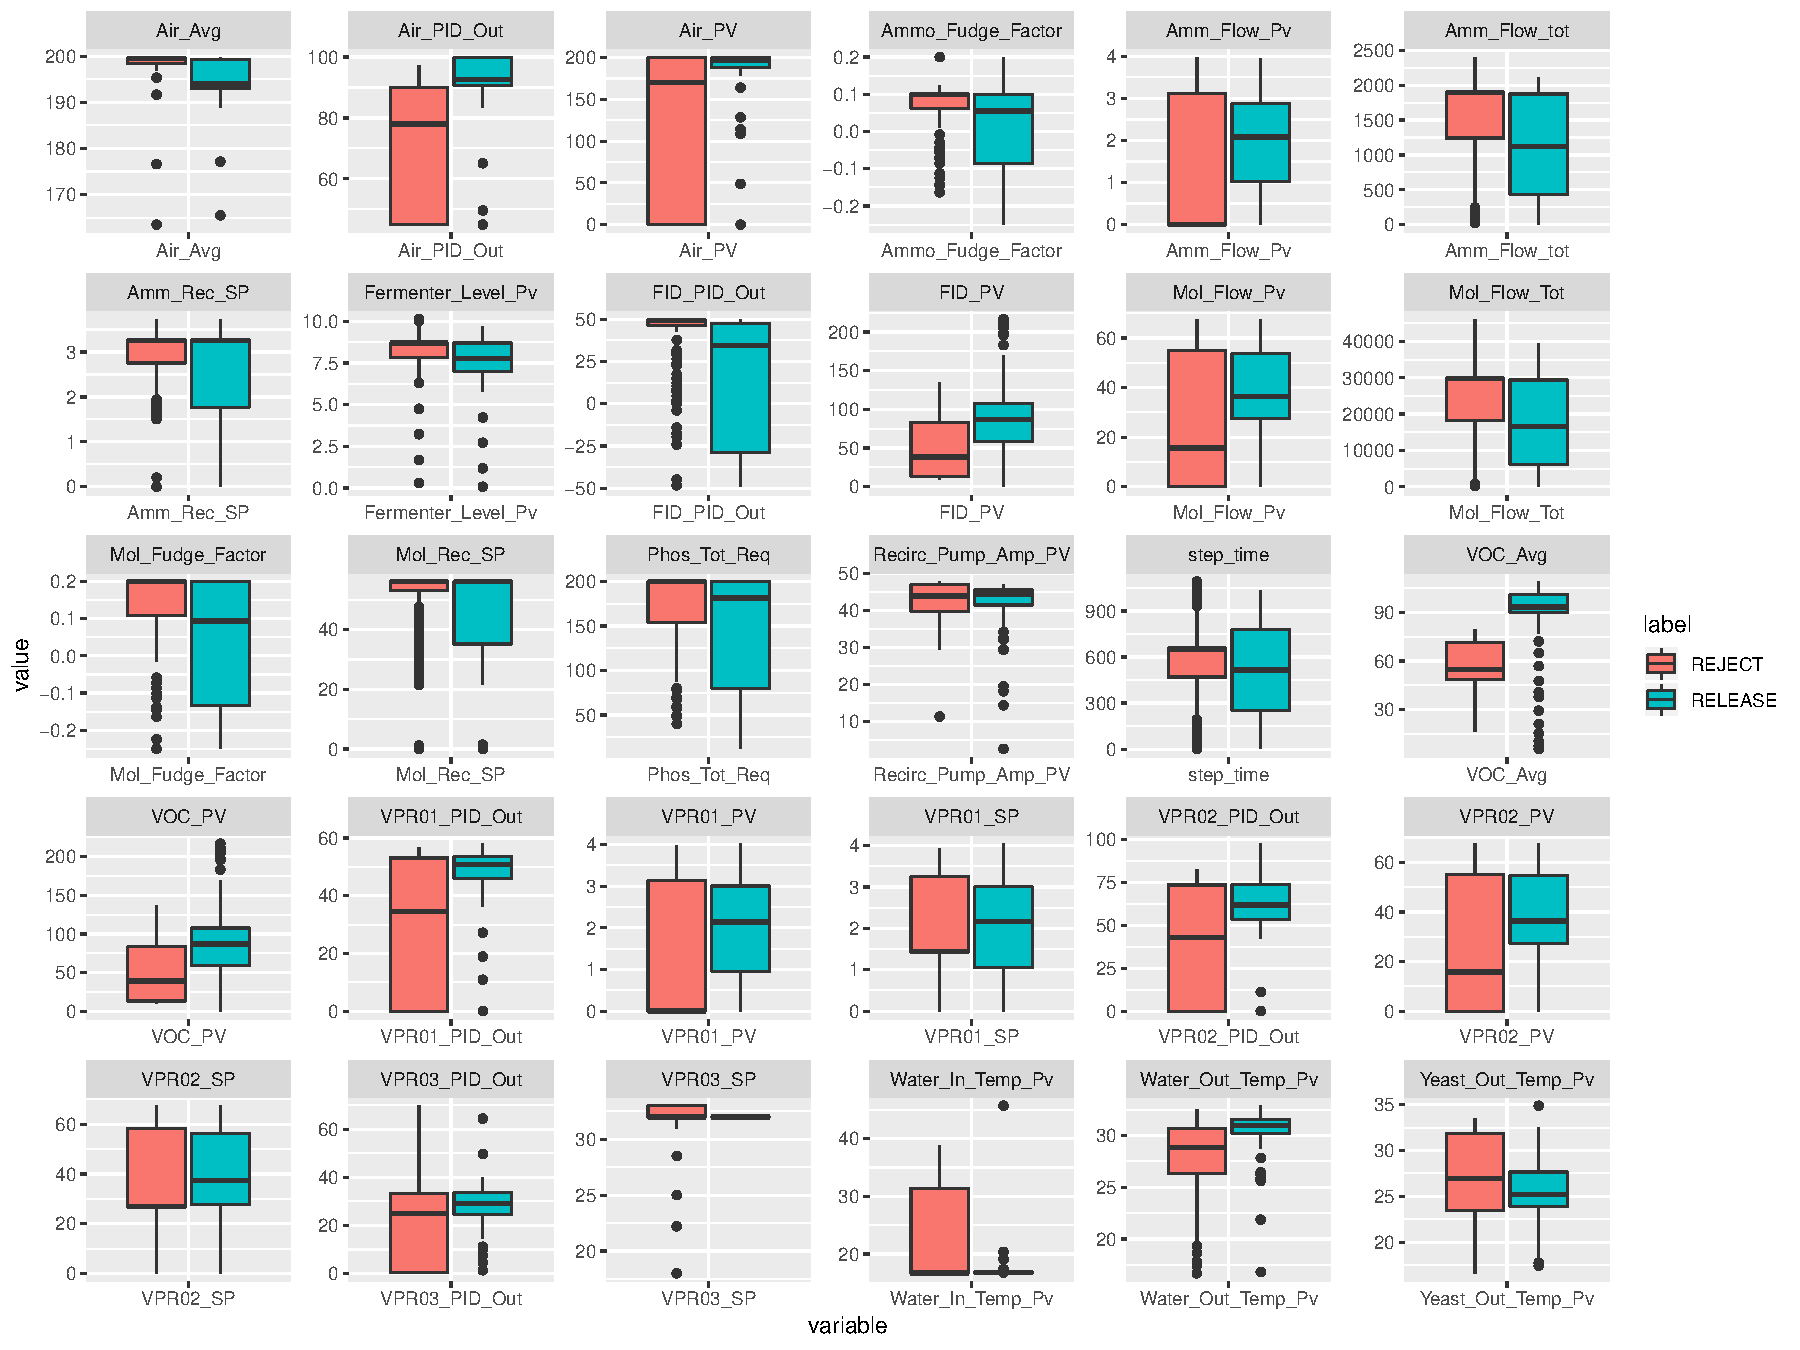
\includegraphics[width=1.0\textwidth]{plots/f5-sample.pdf}
    \caption{F5 sample}
    \label{fig:f5_sample}
\end{figure}

\begin{figure}[ht]
    \centering
    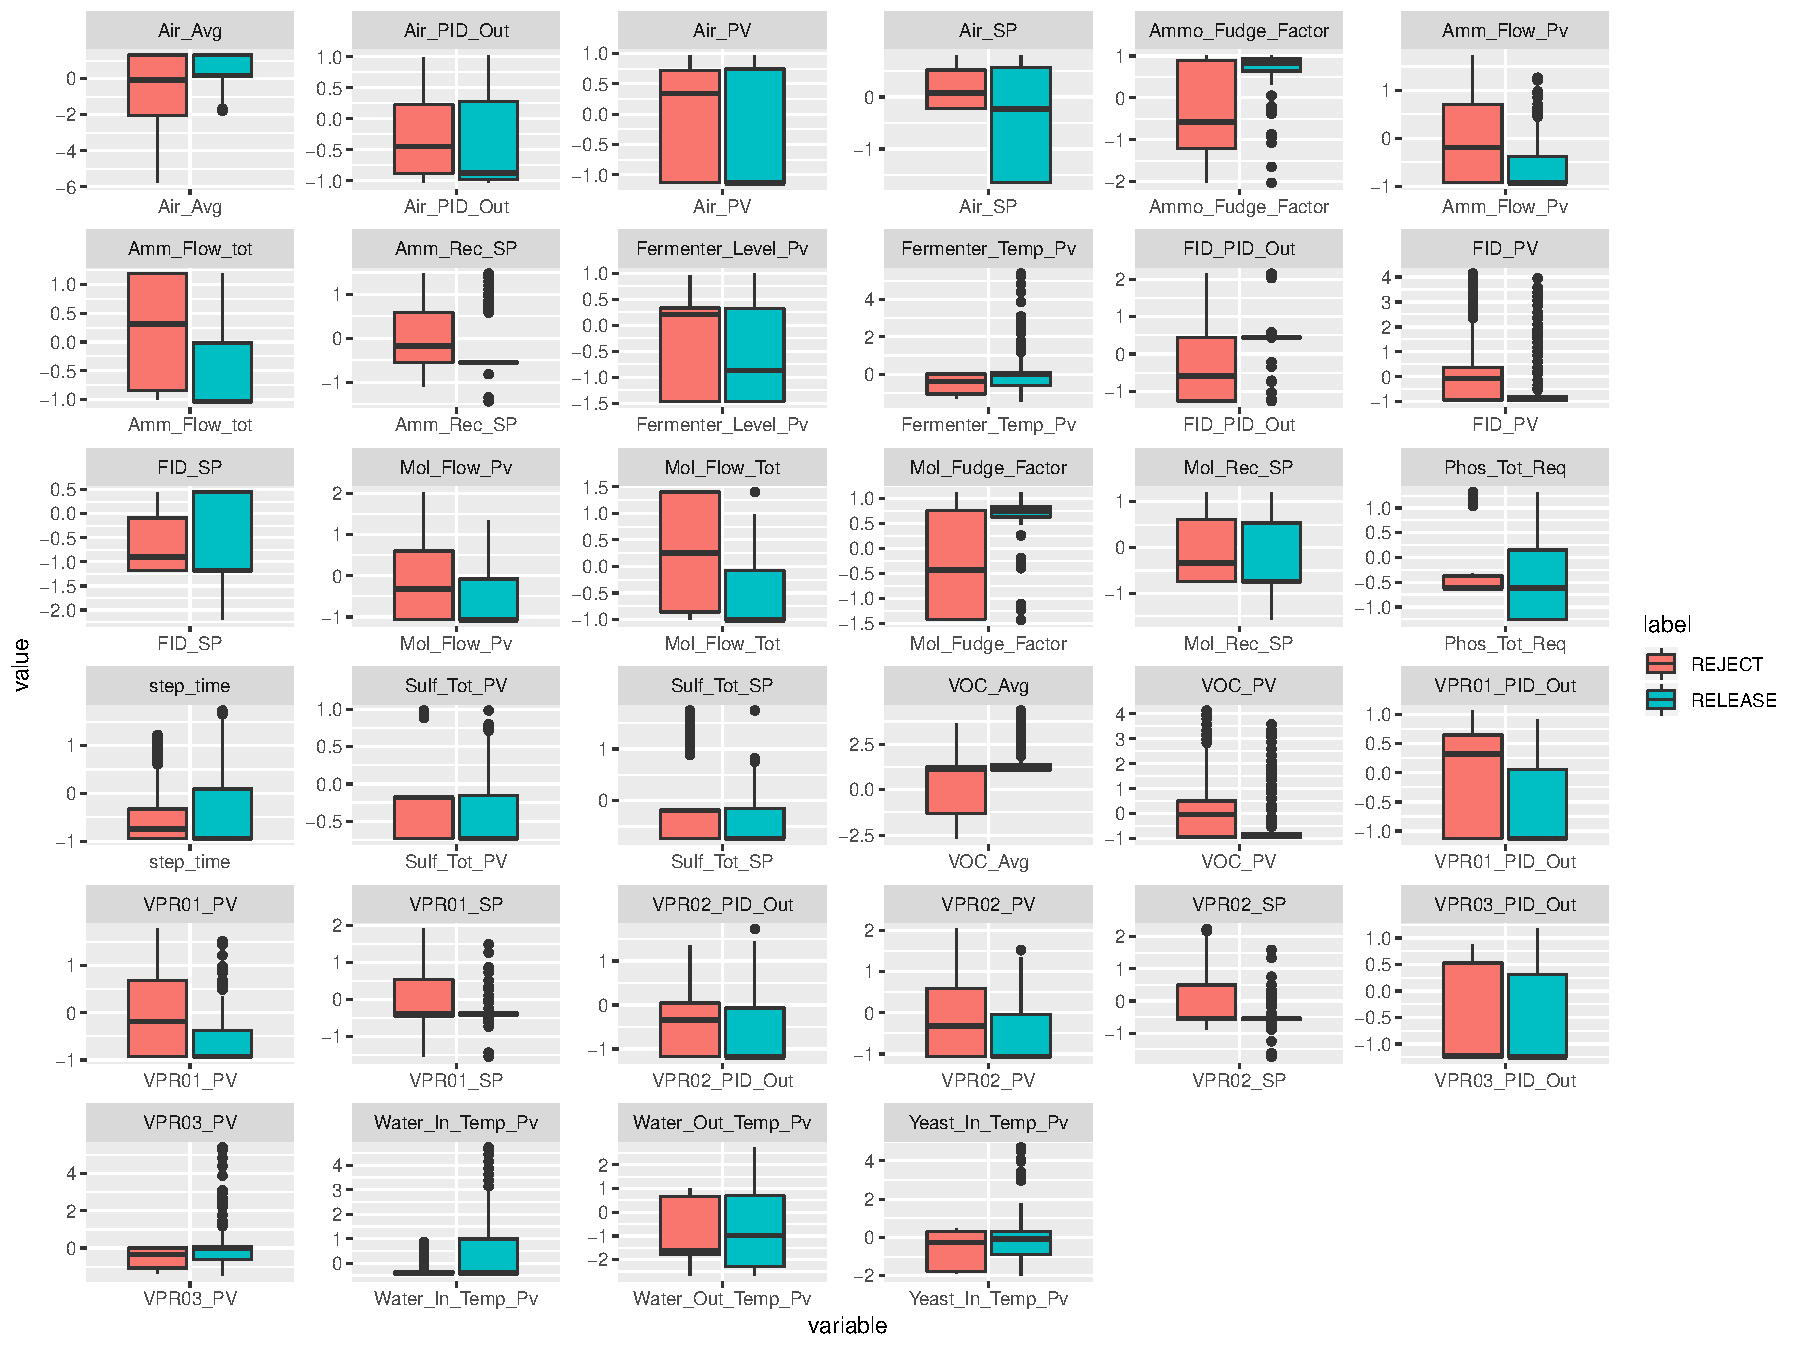
\includegraphics[width=1.0\textwidth]{plots/f5-predicted.pdf}
    \caption{F5 predicted}
    \label{fig:f5_predicted}
\end{figure}

After performing the feature reduction and cluster analysis (PCA and LDA respectively), the lack of data was again evident. When investigating the effectiveness of feature reduction (see Figure \ref{fig:f5_variables}) then, clustering of variables, albeit present, is weak. 

\begin{figure}[ht]
\centering
\begin{subfigure}{.3\textwidth}
    \centering
    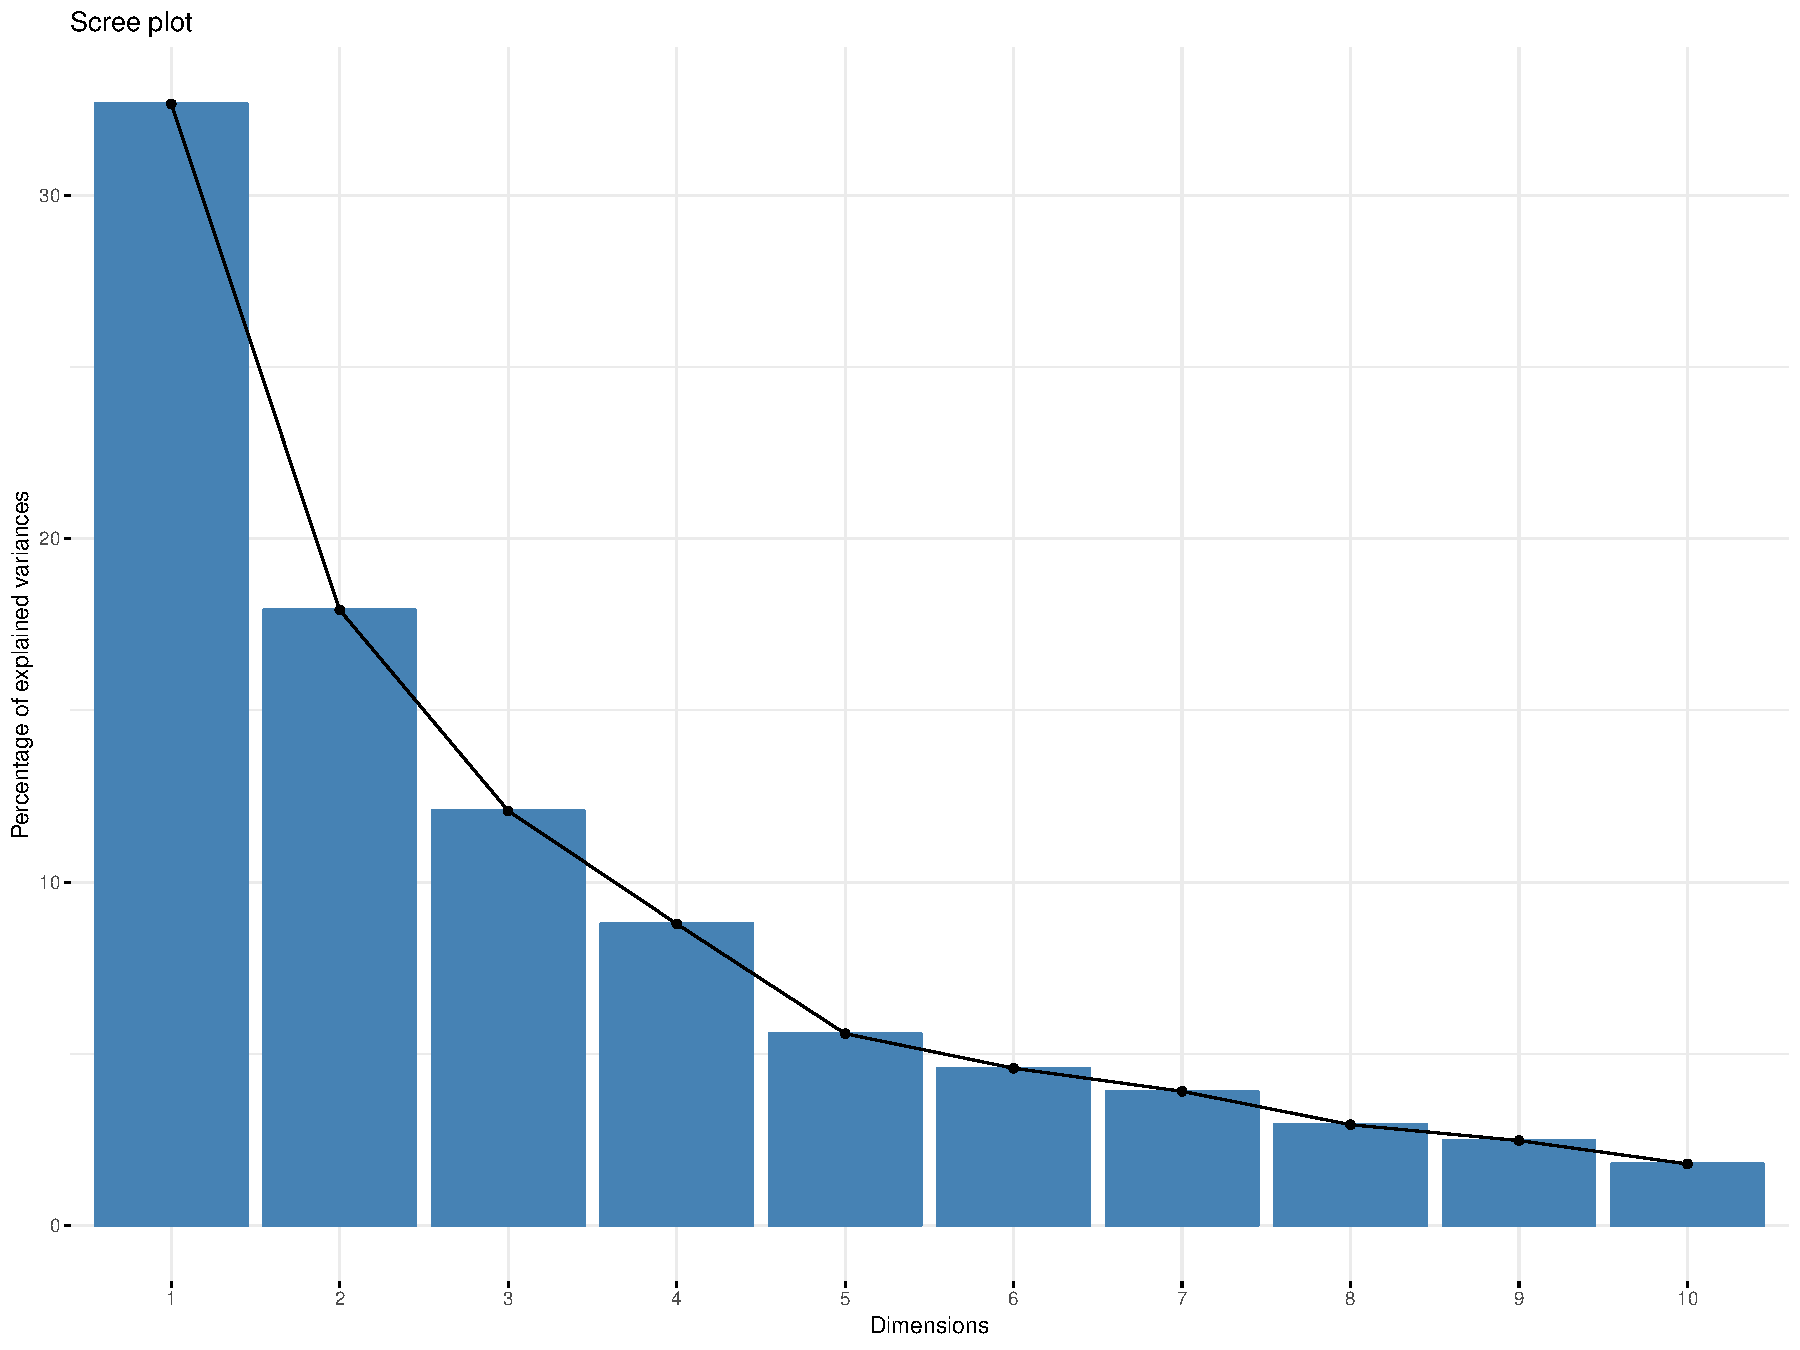
\includegraphics[width=\textwidth]{plots/f5_explained_variances.pdf}        
    \caption{F5 explained variances}
    \label{fig:f5_explained_variances}
\end{subfigure}%
\begin{subfigure}{.3\textwidth}
    \centering
    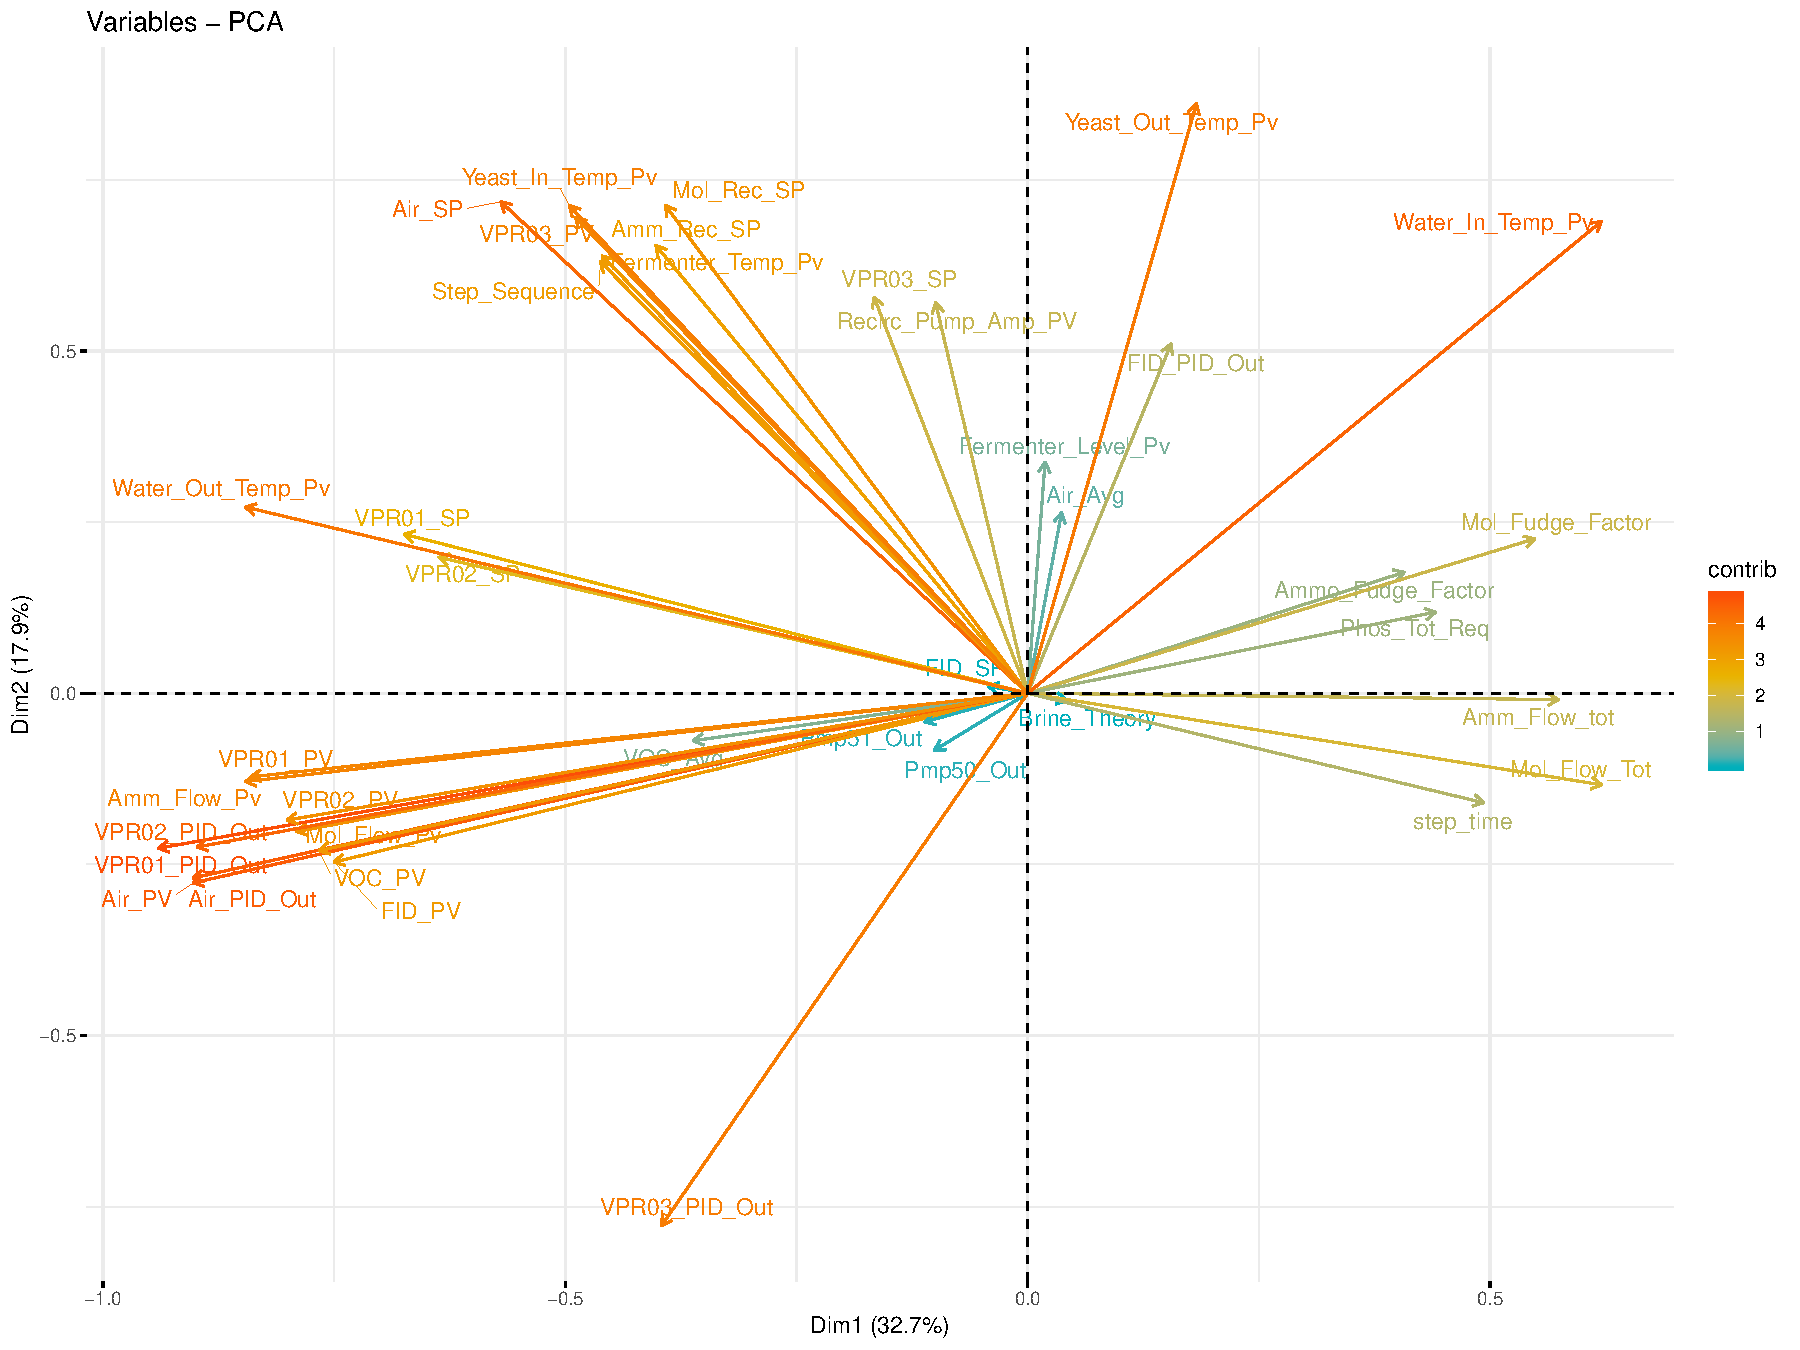
\includegraphics[width=\textwidth]{plots/f5_graph_of_variables.pdf}
    \caption{F5 Variables}
    \label{fig:f5_variables}
\end{subfigure}%
\begin{subfigure}{0.3\textwidth}
    \begin{center}
    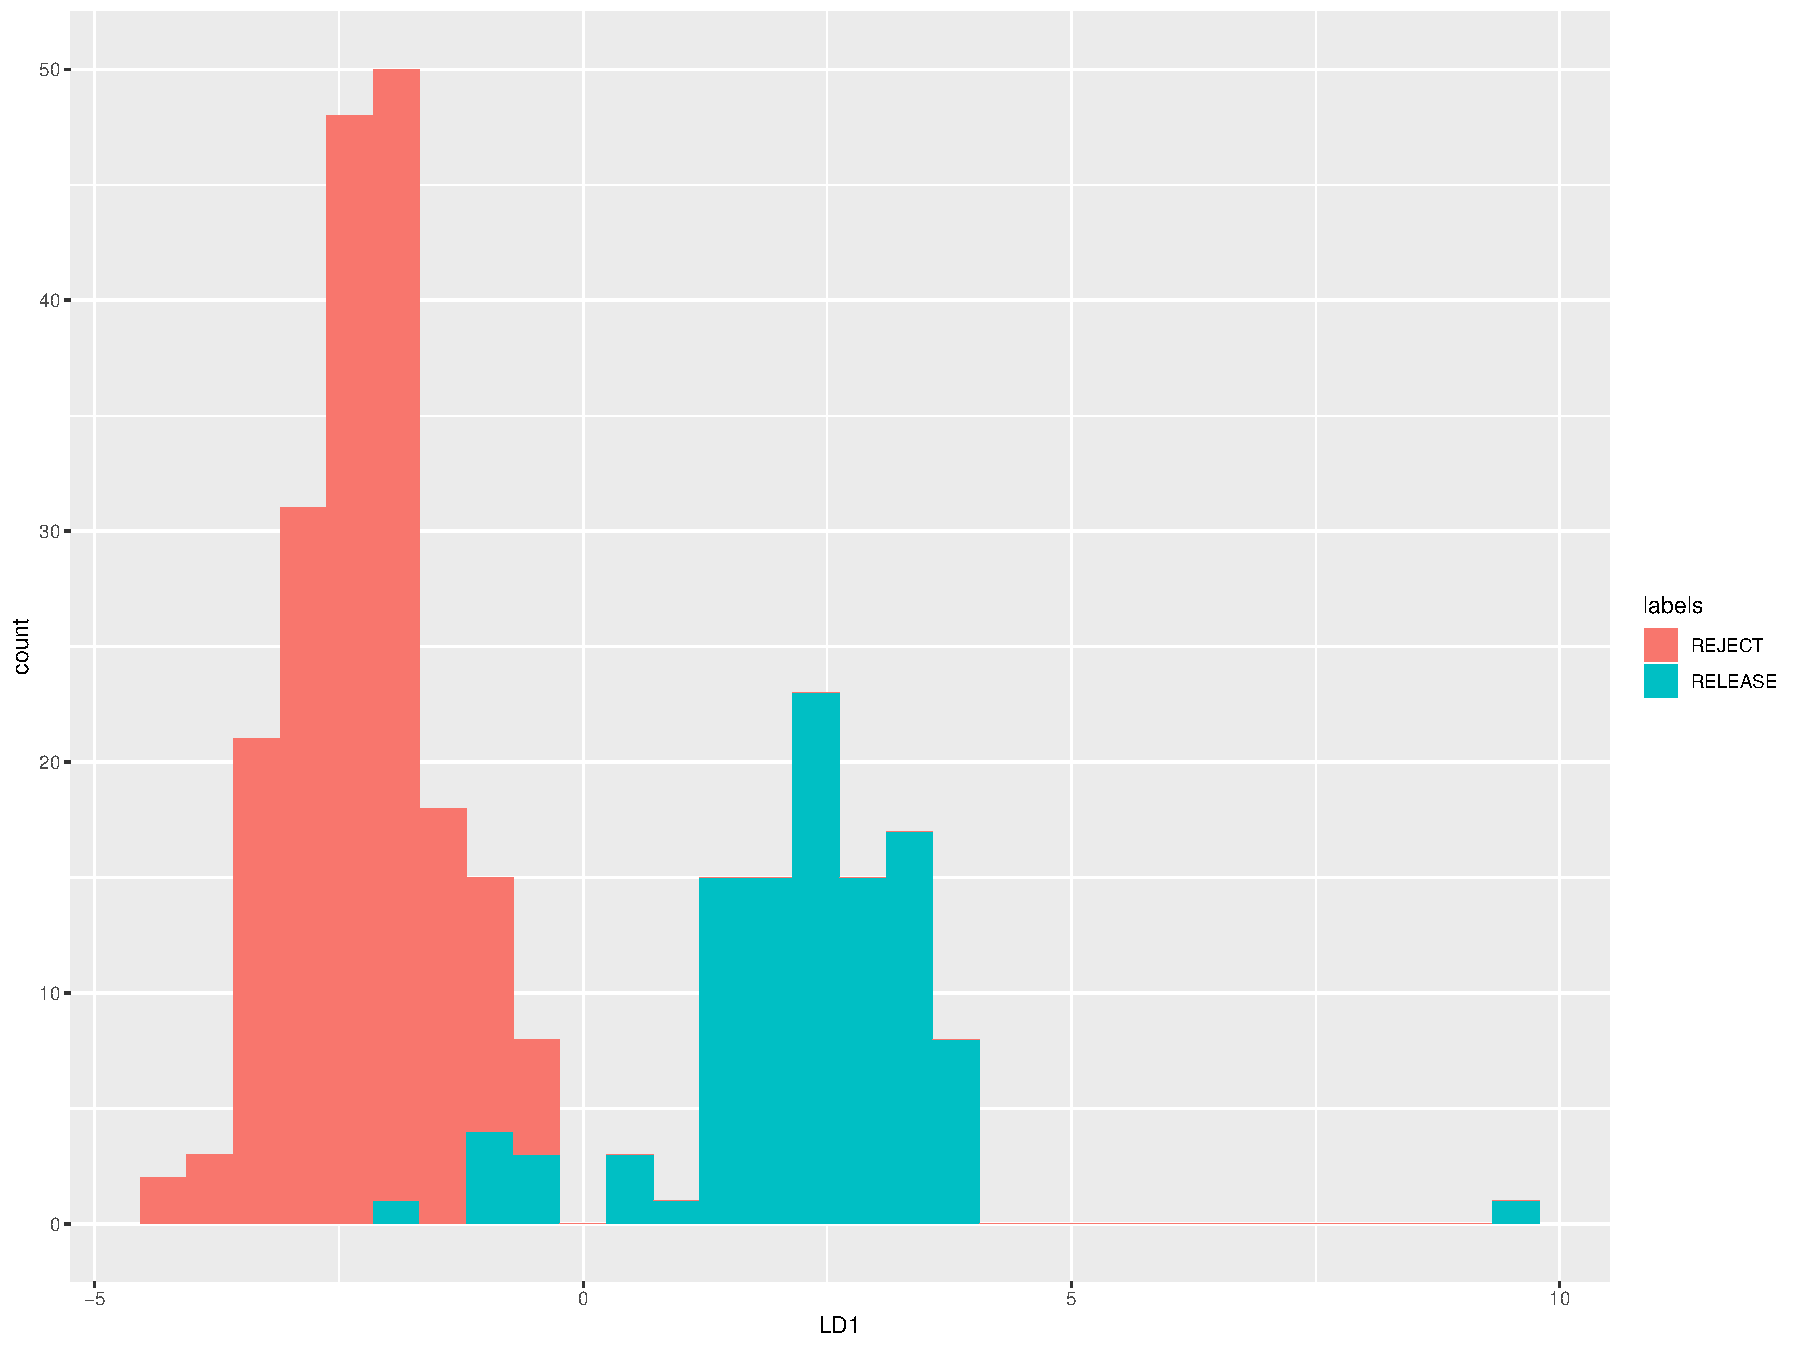
\includegraphics[width=\textwidth]{plots/f5_LD1.pdf}
    \end{center}
    \caption{F5 LD1 distribution across classes}
    \label{fig:f5_LD1}
\end{subfigure}
\end{figure}

The results of LDA are displayed on Figure \ref{fig:f5_LD1}. Even though the Figure shows evidence of strong difference between ``rejected'' and ``released'', it is not reliable since the sample size are one of each class. Therefore the difference between those to production batches could be anything from environment to random chance. More than in any other production step described above, F5 required significant additional data collection to make any substantial conclusions on the process performance and stability.

